% !TEX TS-program = pdflatex
% !TEX encoding = UTF-8 Unicode

% This is a simple template for a LaTeX document using the "article" class.
% See "book", "report", "letter" for other types of document.

\documentclass[11pt]{article} % use larger type; default would be 10pt

\usepackage[utf8]{inputenc} % set input encoding (not needed with XeLaTeX)

%%% Examples of Article customizations
% These packages are optional, depending whether you want the features they provide.
% See the LaTeX Companion or other references for full information.

%%% PAGE DIMENSIONS
\usepackage{geometry} % to change the page dimensions
\geometry{a4paper} % or letterpaper (US) or a5paper or....
% \geometry{margin=2in} % for example, change the margins to 2 inches all round
% \geometry{landscape} % set up the page for landscape
%   read geometry.pdf for detailed page layout information

\usepackage{graphicx} % support the \includegraphics command and options
\graphicspath{ {./Figs/} }  % requires additional {} and trailing '/'!


% \usepackage[parfill]{parskip} % Activate to begin paragraphs with an empty line rather than an indent

%%% PACKAGES
\usepackage{booktabs} % for much better looking tables
\usepackage{array} % for better arrays (eg matrices) in maths
\usepackage{paralist} % very flexible & customisable lists (eg. enumerate/itemize, etc.)
\usepackage{verbatim} % adds environment for commenting out blocks of text & for better verbatim
\usepackage{subfig} % make it possible to include more than one captioned figure/table in a single float

\usepackage{colortbl}
\usepackage{color}
\usepackage{amsmath}
\usepackage{amssymb}
\usepackage{xifthen}
\usepackage{tikz}
\usepackage{relsize}
\usetikzlibrary{matrix}
\usetikzlibrary{positioning}
\usetikzlibrary{calc}
\usetikzlibrary{math}
\usetikzlibrary{shapes}


\usepackage{theorem}
\newtheorem{definition}{Definition}
\newtheorem{proposition}{Proposition}
\newenvironment{proofsketch}{\paragraph{Proof sketch.}}{\hfill$\Box$}

% These packages are all incorporated in the memoir class to one degree or another...

%%% HEADERS & FOOTERS
\usepackage{fancyhdr} % This should be set AFTER setting up the page geometry
\pagestyle{fancy} % options: empty , plain , fancy
\renewcommand{\headrulewidth}{0pt} % customise the layout...
\lhead{}\chead{}\rhead{}
\lfoot{}\cfoot{\thepage}\rfoot{}

%%% SECTION TITLE APPEARANCE
\usepackage{sectsty}
\allsectionsfont{\sffamily\mdseries\upshape} % (See the fntguide.pdf for font help)
% (This matches ConTeXt defaults)

%%% ToC (table of contents) APPEARANCE
\usepackage[nottoc,notlof,notlot]{tocbibind} % Put the bibliography in the ToC
\usepackage[titles,subfigure]{tocloft} % Alter the style of the Table of Contents
\renewcommand{\cftsecfont}{\rmfamily\mdseries\upshape}
\renewcommand{\cftsecpagefont}{\rmfamily\mdseries\upshape} % No bold!

%%% END Article customizations

\newcommand{\ub}{\text{{\tt.}}}

\tikzstyle{bp}=[line width=5pt,draw=blue, opacity=.6,in =90,out=90,looseness=1.5]
\tikzstyle{altbp}=[line width=5pt,draw=red, opacity=.6, in =-90,out=-90,looseness=1.5]
\tikzstyle{cell}=[inner sep=2]
\tikzstyle{backbone}=[line width=2pt]
\tikzstyle{every picture}+=[remember picture]

\def\mySecStr#1{\expandafter {\tt #1}\& }
\def\mySecStrAll#1{\ifx#1\mySecStrAll\else\mySecStr#1\expandafter\mySecStrAll\fi}
\def\mySeq#1{\expandafter {\relsize{-2}\sf #1}\&}
\def\mySeqAll#1{\ifx#1\mySeqAll\else\mySeq#1\expandafter\mySeqAll\fi}


\newcommand{\RNA}[3][]{
\begin{tikzpicture}[baseline={([yshift=-.5ex]rna)}]
  \matrix[matrix of nodes,nodes=cell,ampersand replacement=\&] (rna){
		\mySecStrAll #2 \mySecStrAll\\
		};
\ifthenelse{\equal{#3}{}}{}{%
	\foreach \x/\y in {#3}{\draw (rna-1-\x) edge[bp] (rna-1-\y);}%
}
\ifthenelse{\equal{#1}{}}{}{%
		\foreach \x/\y in {#1}{\draw (rna-1-\x) edge[altbp] (rna-1-\y);}%
		}
\end{tikzpicture}} 

\setlength{\parskip}{1em}
\renewcommand{\H}[1]{{\tt#1}}

\newcommand{\Summary}{
  \tikzstyle{bp}=[line width=5pt,draw=red!50!blue, opacity=.6,in =90,out=90,looseness=1.5]
  \tikzstyle{altbp}=[line width=5pt,draw=red!50!blue, opacity=.6, in =90,out=90,looseness=1.5]
}


\newcommand{\Case}[3]{\item $\{#1\}$: {\sf #3}-type

{\centering 
#2 $\longrightarrow$\Summary#2\\}

}

\newcommand{\SW}[1]{\textbf{SW-}#1}
\newcommand{\YP}[1]{{\color{red!30!black}\textbf{YP-}#1}}

%% band symbols
\newcommand{\Ob}{\text{O}}
\newcommand{\Rb}{\text{R}}
\newcommand{\Lb}{\text{L}}
\newcommand{\Mb}{\text{M}}


%% Matrix symbol macros (from Knotty paper) 
\newcommand{\Vnone}{V}
\newcommand{\V}       [2]{V           (#1,#2)}
\newcommand{\Vhairpin}[2]{V_{\text{hairpin}} (#1,#2)}
\newcommand{\Vstacked}[2]{V_{\text{stacked}} (#1,#2)}
\newcommand{\Viloop}  [2]{V_{\text{iloop}}   (#1,#2)}

\newcommand{\Vhairpins}[2]{V_{\text{hairpin}}^* (#1,#2)}
\newcommand{\Vstackeds}[2]{V_{\text{stacked}}^* (#1,#2)}
\newcommand{\Viloops}  [2]{V_{\text{iloop}}^*   (#1,#2)}

\newcommand{\Vmloopnone}{V_{\text{mloop}}}
\newcommand{\Vmloop}  [2]{V_{\text{mloop}}(#1,#2)}

\newcommand{\pknotnone}{P}
\newcommand{\pknotnones}{\pknotnone^s}
\newcommand{\pknot}[2]{\pknotnone(#1,#2)}

\newcommand {\WMnone}{WM}
\newcommand {\WM}[2]{\WMnone(#1,#2)}
\newcommand {\WMprime}[2]{\WMnone^\prime(#1,#2)}
\newcommand {\WMprimenone}{\WMnone^\prime}

\newcommand {\WBnone}{\mbox{\em WB}}
\newcommand {\WB}[2]{\WBnone(#1,#2)}
\newcommand {\WBprime}[2]{\WBnone^\prime(#1,#2)}
\newcommand {\WBprimenone}{\WBnone^\prime}

\newcommand {\WPnone}{W\!P}
\newcommand {\WP}[2]{\WPnone(#1,#2)}
\newcommand {\WPprime}[2]{\WPnone^\prime(#1,#2)}
\newcommand {\WPprimenone}{\WPnone^\prime}
\newcommand {\WPs}[2]{\WPnone^s(#1,#2)}

\newcommand{\PKnone}{P\!K}
\newcommand {\pk}[4]{\PKnone(#1,#2,#3,#4)}

\newcommand{\PXnone}{P_{X}}
\newcommand {\PX}[4]{\PXnone(#1,#2,#3,#4)}

\newcommand{\PLnone}{P_{\text{L}}}
\newcommand {\PL}[4]{\PLnone(#1,#2,#3,#4)}

\newcommand{\PRnone}{P_{\text{R}}}
\newcommand {\PR}[4]{\PRnone(#1,#2,#3,#4)}

\newcommand{\PMnone}{P_{\text{M}}}
\newcommand {\PM}[4]{\PMnone(#1,#2,#3,#4)}

\newcommand{\POnone}{P_{\text{O}}}
\newcommand {\PO}[4]{\POnone(#1,#2,#3,#4)}

\newcommand{\POSnone}{P_{\text{Os}}}
\newcommand {\POS}[4]{\POSnone(#1,#2,#3,#4)}

\newcommand{\POMnone}{P_{\text{Om}}}
\newcommand {\POM}[4]{\POMnone(#1,#2,#3,#4)}


\newcommand{\PfromLnone}{P_{\text{fromL}}}
\newcommand {\PfromL}[4]{PfromLnone(#1,#2,#3,#4)}

\newcommand{\PfromRnone}{P_{\text{fromR}}}
\newcommand {\PfromR}[4]{P_{\text{fromR}}(#1,#2,#3,#4)}

\newcommand{\PfromMnone}{P_{\text{fromM}}}
\newcommand {\PfromM}[4]{P_{\text{fromM}}(#1,#2,#3,#4)}

\newcommand{\PfromOnone}{P_{\text{fromO}}}
\newcommand {\PfromO}[4]{P_{\text{fromO}}(#1,#2,#3,#4)}

\newcommand{\PfromOMnone}{P_{\text{fromOm}}}
\newcommand {\PfromOM}[4]{P_{\text{fromOm}}(#1,#2,#3,#4)}

\newcommand{\PfromXnone}{P_{\text{from}X}}
\newcommand {\PfromX}[4]{P_{\text{from}X}(#1,#2,#3,#4)}

\newcommand {\wnone}{W}
\newcommand {\w}[2]{W(#1,#2)}
\newcommand {\wm}[2]{\WMnone(#1,#2)}

\newcommand{\VNnone}{V_{\text{N}}}
\newcommand{\WNnone}{W_{\text{N}}}

%% constraints as 'decoration' of matrix symbols
\newcommand{\constrIO} {_\text{O}}
\newcommand{\constrIL} {_\text{L}}
\newcommand{\constrIIO}{_\text{O}}
\newcommand{\constrIIR}{_\text{R}}
\newcommand{\constr}   {_X}

\newcommand{\Pdecomposition}{
  \renewcommand{\GRarcratio}{0.6}
  \renewcommand{\GRsubseqlength}{1}
  \renewcommand{\GRunitlength}{0.1}
  \path[draw=none]
    (last)                node (i1) [label=below:$i_1$] {}
    ++(\GRsubseqlength,0) node (j1) [label=below:$j_1$] {}
    ++(\GRunitlength,0)   node (w1l) [scale=0.1] {}
    ++(\GRdecwfraglength,0)   node (w1r) [scale=0.1] {}
    ++(\GRunitlength,0)   node (i2) [label=below:$i_2$] {}
    ++(\GRsubseqlength,0) node (j2) [label=below:$j_2$] {}
    ++(\GRunitlength,0)   node (w2l) [scale=0.1] {}
    ++(\GRdecwfraglength,0)   node (w2r) [scale=0.1] {}
    ++(\GRunitlength,0)   node (k1) [label=below:$k_1$] {}
    ++(\GRsubseqlength,0) node (l1) [label=below:$l_1$] {}
    ++(\GRunitlength,0)   node (w3l) [scale=0.1] {}
    ++(\GRdecwfraglength,0)   node (w3r) [scale=0.1] {}
    ++(\GRunitlength,0)   node (k2) [label=below:$k_2$] {}
    ++(\GRsubseqlength,0) node (l2) [label=below:$l_2$] {};

  \draw[backbone]
    (i1) edge [] (j1)
    (k1) edge [] (l1)
    (i2) edge [] (j2)
    (k2) edge [] (l2);

  \pgfmathsetmacro\outerradiusX{(4*\GRunitlength+3*\GRsubseqlength+2*\GRdecwfraglength)/2}
  \pgfmathsetmacro\outerradiusY{\outerradiusX*\GRarcratio}
  \pgfmathsetmacro\innerradiusX{(4*\GRunitlength+1*\GRsubseqlength+2*\GRdecwfraglength)/2}
  \pgfmathsetmacro\innerradiusY{\innerradiusX*\GRarcratio}

  \draw
    (w1l) edge [backbone] (w1r)
    (w1l) edge [arc,very densely dashed,out=90,in=90] (w1r)
    (w2l) edge [backbone] (w2r)
    (w2l) edge [arc,very densely dashed,out=90,in=90] (w2r)
    (w3l) edge [backbone] (w3r)
    (w3l) edge [arc,very densely dashed,out=90,in=90] (w3r);

  \draw[arc,very densely dashed]
    (i1) arc [radius=\outerradiusX, y radius=\outerradiusY, start angle=180,end angle=0];
  \draw[arc,very densely dashed]
    (i2) arc [radius=\outerradiusX, y radius=\outerradiusY, start angle=180,end angle=0];
  \draw[arc,very densely dashed]
    (j1) arc [radius=\innerradiusX, y radius=\innerradiusY, start angle=180,end angle=0];
  \draw[arc,very densely dashed]
    (j2) arc [radius=\innerradiusX, y radius=\innerradiusY, start angle=180,end angle=0];
}

%%%%% END matrix symbols/macros


\newcommand{\Def}[1]{\emph{#1}}

%% graphical notation of grammar rules with tikz
\newcommand{\GRgaplength}{0.9}
\newcommand{\GRsubseqlength}{0.35}
\newcommand{\GRarcratio}{0.8}
\newcommand{\GRdecwfraglength}{0.4}
\newcommand{\GRunitlength}{0.15} % distance between concatenated fragments

\tikzstyle{very densely dashed} = [dash pattern=on 2.5pt off 1.5pt]

%% --------------------------------------------------------------------------- 
%% Gapped fragments

% draw base of gapped fragment (without arcs)
\newcommand{\GRgapfragBase}[2][]{%
  \path[draw=none]
    (last)                node (i) [scale=0.1] {}
    ++(\GRsubseqlength,0) node (j) [scale=0.1] {}
    ++(\GRgaplength,0)    node (k) [scale=0.1] {}
    ++(\GRsubseqlength,0) node (l) [scale=0.1] {};
%
  \draw [backbone]
      (i) -- (j)
      (k) -- (l);
%
  \draw (j) edge [draw=none] node [below] (label) {#2} (k); 
%
  \node (last) at (l) {};
}

%draw the points at i,j,k,l for the gapped fragment
\newcommand{\GRgapfragPoints}[1][]{%
  \path[itype/.style=fix,
        jtype/.style=fix,
        ktype/.style=fix,
        ltype/.style=fix,
        #1]
    (i) node [itype] () {}
    (j) node [jtype] () {}
    (k) node [ktype] () {}
    (l) node [ltype] () {};
}

%draw arcs of gapped fragment
\newcommand{\GRgapfragOuterArc}[1]{%
  \pgfmathsetmacro\outerradiusX{(\GRgaplength+2*\GRsubseqlength)/2}
  \pgfmathsetmacro\outerradiusY{\outerradiusX*\GRarcratio}

  \draw[arc,#1]
    (i) arc [radius=\outerradiusX, y radius=\outerradiusY, start angle=180,end angle=0];
}

\newcommand{\GRgapfragInnerArc}[1]{
  \pgfmathsetmacro\innerradiusX{\GRgaplength/2}
  \pgfmathsetmacro\innerradiusY{\innerradiusX*\GRarcratio}
  \draw[arc,#1]
    (j) arc [x radius=\innerradiusX, y radius=\innerradiusY, start angle=180,end angle=0];
}

% draw dashed inner and outer arcs
\newcommand{\GRgapfragArcs}{%
  \GRgapfragInnerArc{very densely dashed}
  \GRgapfragOuterArc{very densely dashed}
}

%% draw a gapped fragment
\newcommand{\GRgapfrag}[2][]{%
  \GRgapfragBase[#1]{#2}
  \GRgapfragArcs
  \GRgapfragPoints[#1]
}

\newcommand{\GRgapfragArcsL}{%
  \GRgapfragArcs
  \draw (i) edge [in=90,out=90,arc] (j);
}
\newcommand{\GRgapfragArcsM}{%
  \GRgapfragInnerArc{solid}
  \GRgapfragOuterArc{very densely dashed}
}
\newcommand{\GRgapfragArcsR}{%
  \GRgapfragArcs
  \draw (k) edge [in=90,out=90,arc] (l);
}
\newcommand{\GRgapfragArcsO}{%
  \GRgapfragInnerArc{very densely dashed}
  \GRgapfragOuterArc{solid}
}

\newcommand{\GRgapfragArcsfromL}{%
  \GRgapfragArcs
  \draw (i) edge [in=90,out=90,arc,dotted] (j);
}
\newcommand{\GRgapfragArcsfromM}{%
  \GRgapfragInnerArc{dotted}
  \GRgapfragOuterArc{very densely dashed}
}
\newcommand{\GRgapfragArcsfromR}{%
  \GRgapfragArcs
  \draw (k) edge [in=90,out=90,arc,dotted] (l);
}
\newcommand{\GRgapfragArcsfromO}{%
  \GRgapfragInnerArc{very densely dashed}
  \GRgapfragOuterArc{dotted}
}

\newcommand{\GRsingleOfrag}{%
  \path[draw=none]
    (last)                node (i) [scale=0.1] {}
    ++(\GRsubseqlength,0) node (j) [scale=0.1] {}
    ++(\GRgaplength,0)    node (k) [scale=0.1] {}
    ++(\GRsubseqlength,0) node (l) [scale=0.1] {};

  \GRgapfragOuterArc{solid}

  \path[itype/.style=fix,
        ltype/.style=fix]
    (i) node [itype] () {}
    (l) node [ltype] () {};
}

\newcommand{\GRgapfragDecorate}{%
}

\newcommand{\GRgapfragDecoratelO}{%
  \pgfmathsetmacro\radiusX{(\GRgaplength+1.5*\GRsubseqlength)/2}
  \pgfmathsetmacro\radiusY{\radiusX*\GRarcratio}
  \draw (i) [arc] arc [x radius=\radiusX, y radius=\radiusY, start angle=180,end angle=0];
}

\newcommand{\GRgapfragDecorateLo}{%
  \pgfmathsetmacro\radiusX{(0.6*\GRsubseqlength)/2}
  \pgfmathsetmacro\radiusY{\radiusX*\GRarcratio}
  \draw (i) [arc] arc [x radius=\radiusX, y radius=\radiusY, start angle=180,end angle=0];
}

\newcommand{\GRgapfragDecoraterO}{%
  \pgfmathsetmacro\radiusX{(\GRgaplength+1.5*\GRsubseqlength)/2}
  \pgfmathsetmacro\radiusY{\radiusX*\GRarcratio}
  \draw (l) [arc] arc [x radius=\radiusX, y radius=\radiusY, start angle=0,end angle=180];
}

\newcommand{\GRgapfragDecorateRo}{%
  \pgfmathsetmacro\radiusX{(0.6*\GRsubseqlength)/2}
  \pgfmathsetmacro\radiusY{\radiusX*\GRarcratio}
  \draw (l) [arc] arc [x radius=\radiusX, y radius=\radiusY, start angle=0,end angle=180];
}

\newcommand{\GRgapfragDeco}[4][]{%
  \GRgapfragBase{#2}
  \csname GRgapfragArcs#3\endcsname
  \csname GRgapfragDecorate#4\endcsname
  \GRgapfragPoints[#1]
}

\newcommand{\GRdecwfrag}[2][]{%
  \path%
    (last) node [scale=0.1]    (i) {}%
    ++(\GRdecwfraglength,0) node [scale=0.1] (l) {};%
  % 
  \draw[very densely dashed,thick] (i) arc (180:0:0.2);%
  %
  \draw [backbone,
        itype/.style={draw=none},
        ltype/.style={draw=none},
        label/.style={below},
        #1]
        (i) node [itype] () {} 
        -- node [label] (label){#2} ++ (0.4,0) 
        node [ltype] () {};%
  \node (last) at (l) {};%
}

\newcommand{\GRsetlast}[2][0]{%
  \path (last) node (bkplast) {}%
    (#2) ++(#1,0) node (last) {};%
}
\newcommand{\GRrestorelast}{%
  \path (bkplast) node (last) {};%
}
\newcommand{\GRconcat}{%
  \path (last) ++(\GRunitlength,0) node (last) {};
}
\newcommand{\GRconcatWAfter}[1]{%
  \GRsetlast[\GRunitlength]{#1}%
}
\newcommand{\GRconcatWBefore}[1]{%
  \pgfmathsetmacro\offset{\GRdecwfraglength+\GRunitlength}
  \GRsetlast[-\offset]{#1}%
}

\newcommand{\GRnewrule}{%
  \path (start) ++(0,-1.5) node (last) {}%
        (last) node (start) {};%
}

% secondary label
\newcommand{\GRseclabel}[1]{%
  \path (l) + (-0.4,0.6) node [text ragged,anchor=west,align=left] (label) {#1};%
  \path (label.east) ++ (-0.2,-0.6) node (last) [] {};%
}

\newcommand{\GRdecompTo}{%
  \draw (last) ++(0.2,0.3) edge [->,very thick] ++(0.9,0);
  \path (last) ++(1.4,0) node (last) {};
}

\newcommand{\GRor}{%
  \draw (last) ++(0.3,0) edge [very thick] ++(0,0.8);
  \path (last) ++(0.6,0) node (last) {};
}


\newenvironment{GRule}{%
  \begin{tikzpicture}[fix/.style={fill,circle,scale=0.4,red!50!black!90},
                      free/.style={fill,rectangle,scale=0.55,blue!60!black!80},
                      backbone/.style={very thick},
                      arc/.style={thick}]
  \node (start) at (0,0) {};
  \node (last) at (0,0) {};
}{%
  \end{tikzpicture}%
}


%%% The "real" document content comes below...

\title{A sketch of unambiguous DP for CCJ}
\author{Hosna, Sebastian, Yann}
%\date{} % Activate to display a given date or no date (if empty),
         % otherwise the current date is printed 



\begin{document}
\maketitle

\textcolor{red}{\textbf{SW - Disclaimer:} Currently, Sections 1 is quite unsorted. Section 1 still contains useful material but some parts may be outdated. Thus, it makes more sense to go through Section 2. In Section 2, I started over again, since I currently think, we should argue about Band-Decomposition-Orders (BDOs) of 'closed' structures over gapped regions (corresponding to $P_X$-fragments) as well as 'closed' pseudoknotted structures over un-gapped regions (corresponding to $P$-fragments). 'Closed' should be defined as a structure that can be reduced only by eating off crossing bands (in the gapped case) or decomposing into two gapped fragments (in the ungapped case); my intuition here is the analogy to closed structures in the non-crossing case, which are the structures that are 'closed' by a base pair.}

\textcolor{red}{%
Section 2 still needs elaboration (of course, final presentation needs a lot of improvements) and merge with Sec 1. For example, Section 1 currently gives rules only for $P_{L/R/M/O}$ whereas we additionally need matrices/states for certain BDO prefixes. The transition diagram of Eq.~(\ref{eq:transitions}) provides the quickest overview, but is certainly not immediately clear without context.}

{\bf TODO}
\begin{itemize}
  \item Technical introduction: Basic definitions for the sake of self-completeness; (Hosna)
  \item Elaborate formal outline of the unambigous decomposition. 
  \item Expand full set of rules, Revise pictures $\to$ TikZ; (Sebastian)
  \item Completeness using generating functions (see Nebel's 2012 JCB paper); (Yann)
  \item Unambiguity through disjointness of produced subsets; (At later time, once complete rules are known)
  \item Applications: 
   \begin{itemize}
    \item Tools: Statistical sampling (à la Ding-Lawrence), Inside-Outside for exact BP prob computation
    \item Tasks: Structure prediction (through Sampling-Clustering) possibly SHAPE directed, Pseudoknot detection (through comparing partition functions), Interaction prediction, kinetics (far-fetched?)...
    \item Target (journals): Sebastian says 'NAR' or 'RNA', Hosna says whatever (I am fine with Bioinformatics or RNA), Yann, uncharacteristically, doesn't say anything...
  \end{itemize}
\end{itemize}


% The original DP decomposition underlying the CCJ algorithm is ambiguous on multiple levels.
% {\em Can we lift this ambiguity without too much hassle?}
% A key element in the decomposition, and one of the major source of ambiguity, resides in the assembly of two \emph{gapped} pseudoknotted elements, akin to the 3-band/kissing hairpin motif. However, in order to achieve maximum expressivity, only the middle helix is mandatory within each gapped element, meaning that some structure may be obtained in several different ways. In this short note, we explore the different combinations, and build a minimal subset of structures, built from combinations of atomic gapped structures that captures the same search space within inducing any ambiguity.

% Let us first introduce a bit of nomenclature. The helices in the first gapped structure are named \H{1}, \H{2} and \H{3} (resp. \H{A}, \H{B} and \H{C}), as illustrated below:

% {\centering 
% \RNA[4/6,5/11,10/12]{121ABA323CBC}{1/3,2/8,7/9}\\}

% \noindent Note that each helix must contain at least one base pair and, in the case where it contains internal loops and recursive subtructures\footnote{Are those allowed anyway?} must start and finish with a base pair (potentially the same if restricted to a single base pair).

% In order to avoid ambiguity at a higher level in the decomposition, it is crucial that the base pairs in the assembly of gapped elements form a unique connected component in the conflict graph induced by the crossing relationship. Indeed, disconnected components correspond to part in a pseudoknot that can be generated either by sequential composition, or by a recursive call, generating a nested subcomponent. It is thus easy to say that helices \H{2} and \H{B} cannot be omitted. Conversely, helices \H{1}, \H{3}, \H{A}, and \H{C} represent leaves of the conflict graph, and can therefore be safely discarded without disconnecting the conflict graph, \emph{i.e.} without inducing any ambiguity.

% We are left to systematically explore the subsets of $\{\H{1}, \H{3}, \H{A}, \H{C}\}$, in combination with the two mandatory helices \H{2} and \H{B}:
% \begin{itemize} 
% \item Second component is $\{\H{B}\}$:
% \begin{itemize} 
% \Case{\H{2}, \H{B}}{\RNA[5/11]{-2--B--2--B-}{2/8}}{H}
% \Case{\H{1},\H{2}, \H{B}}{\RNA[5/11]{121-B--2--B-}{1/3,2/8}}{KH}
% \Case{\H{2}, \H{3}, \H{B}}{\RNA[5/11]{-2--B-323-B-}{2/8,7/9}}{H}
% {\bfseries Note:} Second band features at least 2 base pairs
% \Case{\H{1},\H{2}, \H{3}, \H{B}}{\RNA[5/11]{121-B-323-B-}{1/3,2/8,7/9}}{KH}
% {\bfseries Note:} Third band features at least 2 base pairs
% \end{itemize} 
% \item Second component is $\{\H{A},\H{B}\}$:
% \begin{itemize} 
% \Case{\H{2}, \H{A}, \H{B}}{\RNA[4/6,5/11]{-2-ABA-2--B-}{2/8}}{H}
% {\bfseries Note:} First band features at least 2 base pairs
% \Case{\H{1},\H{2}, \H{A}, \H{B}}{\RNA[4/6,5/11]{121ABA-2--B-}{1/3,2/8}}{KH$^{\text{a}}$}
% \Case{\H{2}, \H{3}, \H{A}, \H{B}}{\RNA[4/6,5/11]{-2-ABA323-B-}{2/8,7/9}}{H$^{\text{a}}$}
% \Case{\H{1},\H{2}, \H{3}, \H{A}, \H{B}}{\RNA[4/6,5/11]{121ABA323-B-}{1/3,2/8,7/9}}{KH$^{\text{b}}$}
% \end{itemize} 
% \item Second component is $\{\H{B},\H{C}\}$:
% \begin{itemize} 
% \Case{\H{2}, \H{B}, \H{C}}{\RNA[5/11,10/12]{-2--B--2-CBC}{2/8}}{KH}
% \Case{\H{1},\H{2}, \H{B}, \H{C}}{\RNA[5/11,10/12]{121-B--2-CBC}{1/3,2/8}}{4B}
% \Case{\H{2}, \H{3}, \H{B}, \H{C}}{\RNA[5/11,10/12]{-2--B-323CBC}{2/8,7/9}}{KH$^{\text{c}}$}
% \Case{\H{1},\H{2}, \H{3}, \H{B}, \H{C}}{\RNA[5/11,10/12]{121-B-323CBC}{1/3,2/8,7/9}}{4B$^{\text{a}}$}
% \end{itemize} 
% \item Second component is $\{\H{A},\H{B},\H{C}\}$:
% \begin{itemize} 
% \Case{\H{2}, \H{A}, \H{B}, \H{C}}{\RNA[4/6,5/11,10/12]{-2-ABA-2-CBC}{2/8}}{KH}
% {\bfseries Note:} First band features at least 2 base pairs
% \Case{\H{1},\H{2}, \H{A}, \H{B}, \H{C}}{\RNA[4/6,5/11,10/12]{121ABA-2-CBC}{1/3,2/8}}{4B$^{\text{b}}$}
% \Case{\H{2}, \H{3}, \H{A}, \H{B}, \H{C}}{\RNA[4/6,5/11,10/12]{-2-ABA323CBC}{2/8,7/9}}{KH$^{\text{d}}$}
% \Case{\H{1},\H{2}, \H{3}, \H{A}, \H{B}, \H{C}}{\RNA[4/6,5/11,10/12]{121ABA323CBC}{1/3,2/8,7/9}}{CCJ}
% \end{itemize}
% \end{itemize}

% \begin{table}
% { 
%   \tikzstyle{cell}=[inner sep=1.2]
%   \tikzstyle{bp}=[line width=2pt,draw=red!50!blue!80!white, opacity=1,in =90,out=90,looseness=1.3]
%   \tikzstyle{altbp}=[line width=2pt,draw=red!50!blue!80!white, opacity=1, in =90,out=90,looseness=1.3]
% \centering\begin{tabular}{@{}ll@{}ll@{}l@{}}\toprule
% Type & Helix classes && Subsets (sort of)&\\ \midrule
% {\sf H} & $\{\H{2},\H{B}\}$ &\RNA[5/11]{-2--B--2--B-}{2/8}& $\{\H{2},\H{3},\H{B}\}$&\RNA[5/11]{-2--B-323-B-}{2/8,7/9}\\ 
% & &  & $\{\H{2},\H{A},\H{B}\}$  &\RNA[4/6,5/11]{-2-ABA-2--B-}{2/8}\\ 
% \arrayrulecolor{gray!60}\midrule
% {\sf H}$^{\text{a}}$ & $\{\H{2}, \H{3}, \H{A}, \H{B}\}$&\RNA[4/6,5/11]{-2-ABA323-B-}{2/8,7/9} &  &\\ 
% \arrayrulecolor{black}\midrule
% {\sf KH} & $\{\H{1},\H{2},\H{B}\}$&\RNA[5/11]{121-B--2--B-}{1/3,2/8} & $\{\H{1},\H{2},\H{3},\H{B}\}$  &\RNA[5/11]{121-B-323-B-}{1/3,2/8,7/9}\\ 
%  & $\{\H{2},\H{B},\H{C}\}$ &\RNA[5/11,10/12]{-2--B--2-CBC}{2/8} & $\{\H{2},\H{A},\H{B},\H{C}\}$  &\RNA[4/6,5/11,10/12]{-2-ABA-2-CBC}{2/8}\\ 
% \arrayrulecolor{gray!60}\midrule
% {\sf KH}$^{\text{a}}$ & $\{\H{1},\H{2}, \H{A}, \H{B}\}$&\RNA[4/6,5/11]{121ABA-2--B-}{1/3,2/8} &  & \\ 
% {\sf KH}$^{\text{b}}$ & $\{\H{1},\H{2}, \H{3}, \H{A}, \H{B}\}$&\RNA[4/6,5/11]{121ABA323-B-}{1/3,2/8,7/9} &  &\\ 
% {\sf KH}$^{\text{c}}$ & $\{\H{2}, \H{3}, \H{B}, \H{C}\}$&\RNA[5/11,10/12]{-2--B-323CBC}{2/8,7/9} &  & \\ 
% {\sf KH}$^{\text{d}}$ & $\{\H{2}, \H{3}, \H{A}, \H{B}, \H{C}\}$&\RNA[4/6,5/11,10/12]{-2-ABA323CBC}{2/8,7/9} &  & \\ 
% \arrayrulecolor{black}\midrule
% {\sf 4B} & $\{\H{1},\H{2},\H{B},\H{C}\}$&\RNA[5/11,10/12]{121-B--2-CBC}{1/3,2/8}  &  &\\ 
% \arrayrulecolor{gray!60}\midrule
% {\sf 4B}$^{\text{a}}$ & $\{\H{1},\H{2}, \H{3}, \H{B}, \H{C}\}$&\RNA[5/11,10/12]{121-B-323CBC}{1/3,2/8,7/9} &  & \\ 
% {\sf 4B}$^{\text{b}}$ & $\{\H{1},\H{2}, \H{A}, \H{B}, \H{C}\}$&\RNA[4/6,5/11,10/12]{121ABA-2-CBC}{1/3,2/8} &  & \\ 
% \arrayrulecolor{black}\midrule
% {\sf CCJ} & $\{\H{1},\H{2},\H{3},\H{A},\H{B},\H{C}\}$&\RNA[4/6,5/11,10/12]{121ABA323CBC}{1/3,2/8,7/9} &  &\\ 
% \bottomrule
% \end{tabular}\\}

% \caption{Isomorphism classes for relevant subsets of {\sf CCJ} helices}\label{tab:iso}
% \end{table}

% We summarize in Table~\ref{tab:iso} the various accessible classes. A close inspection of the classes reveals two -- complete and unambiguous -- decompositions of the CCJ class in the following subsets of non-empty helices:

% {\centering$\{\H{2},\H{B}\}$, 
% $\{\H{2}, \H{3}, \H{A}, \H{B}\}$, 
% $\{\H{1},\H{2},\H{B}\}$ \emph{or} $\{\H{2},\H{B},\H{C}\}$,
% $\{\H{1},\H{2}, \H{A}, \H{B}\}$,
% $\{\H{1},\H{2}, \H{3}, \H{A}, \H{B}\}$,
% $\{\H{2}, \H{3}, \H{B}, \H{C}\}$,
% $\{\H{2}, \H{3}, \H{A}, \H{B}, \H{C}\}$,
% $\{\H{1},\H{2},\H{B},\H{C}\}$,
% $\{\H{1},\H{2}, \H{3}, \H{B}, \H{C}\}$,
% $\{\H{1},\H{2}, \H{A}, \H{B}, \H{C}\}$,
% $\{\H{1},\H{2},\H{3},\H{A},\H{B},\H{C}\}$\\}

% From this partition of the search space for canonical CCJ pseudoknots, one obtains a complete/unambiguous, if definitely tedious, decomposition:
% \newcommand{\Basic}{
%   \tikzstyle{bp}=[line width=20pt,draw=blue!50!red!80, opacity=.6, in=90, out=90,looseness=2]
%   \tikzstyle{altbp}=[line width=20pt,draw=blue!50!red!80, opacity=.6, in=-90, out=-90,looseness=2]
%   \tikzstyle{cell}+=[inner sep=8pt]
% }
% \newcommand{\RHS}[2]{{\Basic
%   \tikzstyle{bp}+=[draw=blue]
%   \tikzstyle{altbp}+=[draw=red]
% \RNA[2/4]{----}{1/3}
% \tikz[overlay]{
% \node[above=17.5pt of rna-1-2,inner sep=2pt,fill=blue!10,rounded corners=3pt]{\H{#1}};
% \node[below=17.5pt of rna-1-3,inner sep=2pt,fill=red!10,rounded corners=3pt]{\H{#2}};
% \draw[backbone] (rna-1-1.west) edge (rna-1-4.east); 
% \node[below=1pt of rna-1-1.north west,inner sep=0]{$i$};
% \node[below=1pt of rna-1-1.north east,inner sep=0]{$k$};
% \node[above=1pt of rna-1-2.south west,inner sep=0]{$k$+$1$};
% \node[above=1pt of rna-1-2.south east,inner sep=0]{$l$};
% \node[below=1pt of rna-1-3.north west,inner sep=0]{$l$+$1$};
% \node[below=1pt of rna-1-3.north east,inner sep=0]{$m$};
% \node[above=1pt of rna-1-4.south west,inner sep=0]{$m$+$1$};
% \node[above=1pt of rna-1-4.south east,inner sep=0]{$j$};

% }}}
% \begin{align*}
% {\Basic\RNA[2/4]{----}{1/3}
% \tikz[overlay]{
% \node[below=-2pt of rna-1-1.south west,inner sep=0]{$i$};
% \node[above=-2pt of rna-1-4.north east,inner sep=0]{$j$};
% \draw[backbone] (rna-1-1.west) edge (rna-1-4.east); 
% }}  \to &\RHS{2}{B} + \RHS{2,3}{A,B} + \RHS{1,2}{B}\\
% +&\RHS{1,2}{A,B}+\RHS{1,2,3}{A,B}+\RHS{2,3}{B,C}\\
% +&\RHS{2,3}{A,B,C}+\RHS{1,2}{B,C}+\RHS{1,2,3}{B,C}\\
% +&\RHS{1,2}{A,B,C}+\RHS{1,2,3}{A,B,C}\\
% \end{align*}
% This decomposition must then be completed with rules for the \emph{gapped} portions, essentially corresponding to constrained versions of rules in the initial {\sf CCJ} algorithm.

\section{Unambiguous decomposition}

\subsection{Preliminaries}

\begin{definition}[Crossing]
if base pairs $i.j$ and $i'.j'$ are in the structure, $R$, and $i<i'<j<j'$, we say that pair $i.j$ crosses pair $i'.j'$ from the left (and $i'.j'$ crosses $i.j$ from the right).
\end{definition}

\begin{definition}[Region] 
The \emph{region $[i,j]$} is the sequence of indices $k$, $i\leq k\leq j$.
$i$ and $j$ are called the left and right ends of the region respectively. 
\end{definition}

\begin{definition}[Gapped region]
A gapped region is the union of two regions $[i, j]$ and $[k, l]$ with $i \le j<k \le l$.
\end{definition}

\begin{definition}[Span the gapped region]
Base pair $d.e$ spans gapped region $[i, j] \cup [k, l]$ if $d \in [i, j]$ and $e \in [k, l]$.

\end{definition}

% HJ - Definition is modified from HFold paper.
% This will make sure that our definition of the band includes the nested unpaired bases as well as any nested substructures.
\textbf{HJ-}  Let $i.j$ and $i'.j'$ be the first and the last base pairs in a maximal 
chain of $\preceq$ while they all cross the same band. Then, $[i,i'] \cup [j',j]$ is a \emph{band}. 
We call $[i,i']$ and $[j',j]$ the band regions, 
and call $i'.j'$ and $i.j$ the inner and outer base pairs of the band respectively.

\SW{There is a subtle detail whether the base pairs of a band have to form a chain of directly nested base pairs. I try to re-define bands more precisely in the following. Feel free to correct me.}

Two base pairs $(i,j)$ and $(i',j')$ are \emph{nested} iff $i<i'<j'<j$ or $i'<i<j<j'$; they cross iff $i<i'<j<j'$ or $i'<i<j'<i'$. In a structure $R$, we call $(i',j')$ directly nested in $(i,j)$ iff $i<i'<j'<j$ and there is no base pair $(i'',j'')\in R$  $i<i''<i'<j'<j''<j$.

\begin{definition}[Band]
A \emph{band} $B$ of a structure $R$ is a set of sequence positions with the following properties:
\begin{itemize}
\item $B=[i,j]\cup[k,l]$, ($i\leq j, j<k-1, k\leq l$)
\item $i.l$ and $j.k$ are base pairs of $R$, the \emph{closing base pairs of $B$}.
\item Define the \emph{base pairs of $B$} as the base pairs of $R$
in the chain $i.l=i_1.j_1, \dots, i_q.j_q=j.k$, where all successive base pairs are directly nested.
 Each base pair in $R$ either crosses all or none of the base pairs of $B$. 
\item $B$ is (set inclusion) maximal, subject to the preceeding properties.
\end{itemize}
\end{definition}

In a RNA structure $R$, the band $[i,j]\cup[k,l]$ is called \emph{band of the base pair $x.y$}, iff $x\in[i,j]$ and $y\in[k,l]$. We emphasize that in this way each base pair uniquely determines a corresponding band (in a given RNA structure).

\SW{It seems simpler to start over based on my first definition:}

Bands are equivalently defined as follows:

\begin{definition}[Band]
For an RNA structure $R$, a \emph{base pair band $\cal B\subseteq R$} is a maximal set of base pairs that 1) form a chain of directly nested base pairs, and where 2) each base pair in $R$ either crosses all or no base pairs in $\cal B$.

A \emph{band} is a subset $[i,j]\cup[k,l]$ of sequence positions, iff there is a base pair band, such that its outermost base pair is $i.l$ and its innermost base pair is $j.k$.
\end{definition}
\textbf{HJ-} We say a base pair $d.e$ spans the band if it spans the gapped region $[i,j]\cup[k,l]$.



\subsection{Methods}

\SW{I try to make clear how I understand the terms 'fragment' and 'rule':}

We decompose classes of structures recursively, starting with the set of all CCJ-structures of the region $[1,n]$ (i.e. the entire sequence). 
In the course of the recursive decomposition, we decompose sets of structures over gapped and ungapped regions. These sets are specific sub-classes of the CCJ structures over the region, which are defined by a number of additional properties (aka constraints) on the structures, like ``there must be a base pair $i.l$''.
In the following, we use the terms \Def{(gapped/ungapped) fragment of type $T$}, briefly \Def{$T$-fragment}, referring to a (respectively, gapped/ungapped) region together with a type $T$, associated with a specific set of constraints on the structures of the $T$-fragment. Thus, $T$-fragments define a very specific set of RNA structures over the region of the fragment, which exists of all CCJ-structures that satisfy the $T$-associated constraints.

Generally we formulate $T$-rules to describe the decomposition of $T$-fragments.
Arbitrary CCJ-structures are decomposed unambiguously due to
\begin{equation}
  \label{eq:wrule}
  
\includegraphics{KnottyPF/recursionW}
\end{equation}
In this graphical notation, the RNA sequence is represented as a line with bases as index positions. This specifies the region of each fragment.
%
Red circles represent fixed end points of a region. Blue squares are free indices (i.e. bases that are pivotal for boundary determinations). 
To not clutter the representation, we do not mark end points that can be identified from bases directly before or after them.
We annotate the fragments by their types (here, $W$, $V$, and $P$) and use \Def{decorations} to indicate the type. Such decorations, e.g. by solid arcs or dashed arcs, serve as mnemonics for the properties of the respective fragments; e.g. we use solid arcs to indicate base pairs like in the $V$-fragment, where all structures must pair the two ends, and dashed arcs to indicate the presence of some structure below the arc, as in $W$-fragments.

\YP{Regarding graphical notations, I think it would be better to use 'wavy line' instead of dashed base pairs in order to better distinguish recursive calls from arcs.}\SW{Sure, we can have wavy lines; it's a simple change for the tikz-generated graphics; I even tested this already. Currently, unfortunately not all of the rules are TikZ, such that I would postpone this. Also, I am not super-convinced that this makes things clearer (it looks more fancy though).}

Similar changes disambiguate the WB and WP recursions. 
This moves the focus to the decomposition of $P$-fragments. 

%\textbf{HJ-} I think we should use $P$-rule instead.
$P$-fragments represent structures $R$ of regions $[i,l]$, where
$i$ and $l$ are paired and part of the same pseudoknot, i.e. in all those structures, there are base pairs $i.i'$ and $l'.l$, such that
\begin{enumerate}
\item either $i.i'$ and $j.j'$ directly cross each other 
\item or $i.i'$ and $l'.l$ are both crossing a third base pair $(k,k')$, where $i<k<i'<l'<k'<l$.
\item $i.i'$ crosses a base pair $(k_1,k_1')$ that crosses $(k_2,k'_2)$ that crosses $l'.l$ $(i<k_1<k_2<k'_1<k'_2<l)$.
\end{enumerate}

Therefore, we distinguish three corresponding cases for their decomposition:
\begin{equation}
\renewcommand{\GRsubseqlength}{0.5}
%
\begin{GRule}
\GRgapfrag[jtype/.style=free,ktype/.style=free,ltype/.style=free]{}{}{lO}
\pgfmathsetmacro\radiusX{(\GRgaplength+1.5*\GRsubseqlength)/2}
\pgfmathsetmacro\radiusY{\radiusX*\GRarcratio}
\draw[red] (i) [arc] arc [x radius=\radiusX, y radius=\radiusY, start angle=180,end angle=0];
%
\path (last) ++(0.7,0) node (last) {};
\begin{scope}[rotate=180]
  \GRgapfrag[jtype/.style={draw=none},ktype/.style={draw=none},ltype/.style={draw=none}]{}{}{}
  \draw[red] (i) [arc] arc [x radius=\radiusX, y radius=\radiusY, start angle=180,end angle=0];
\end{scope}
\end{GRule}
%
\qquad
%
\begin{GRule}
\GRgapfrag[jtype/.style=free,ktype/.style=free,ltype/.style=free]{}{}{lO}
\pgfmathsetmacro\radiusX{(\GRgaplength+1.5*\GRsubseqlength)/2}
\pgfmathsetmacro\radiusY{\radiusX*\GRarcratio}
\draw[red] (i) [arc] arc [x radius=\radiusX, y radius=\radiusY, start angle=180,end angle=0];
%
\path (last) ++(0.7,0) node (last) {};
\begin{scope}[rotate=180]
  \GRgapfrag[jtype/.style={draw=none},ktype/.style={draw=none},ltype/.style={draw=none}]{}{}{}
  \pgfmathsetmacro\radiusX{(\GRgaplength+1.5*\GRsubseqlength - 0.15)/2}
  \pgfmathsetmacro\radiusY{\radiusX*\GRarcratio}
  \draw[blue] (i) +(0.15,0) [arc] arc [x radius=\radiusX, y radius=\radiusY, start angle=180,end angle=0];
  %
  \pgfmathsetmacro\radiusX{(0.8*\GRsubseqlength)/2}
  \pgfmathsetmacro\radiusY{\radiusX*\GRarcratio}
  \draw[red] (i) [arc] arc [x radius=\radiusX, y radius=\radiusY, start angle=180,end angle=0];
\end{scope}
\end{GRule}
%
\qquad
%
\begin{GRule}
\GRgapfrag[jtype/.style=free,ktype/.style=free,ltype/.style=free]{}{}{lO}
\pgfmathsetmacro\radiusX{(0.8*\GRsubseqlength)/2}
\pgfmathsetmacro\radiusY{\radiusX*\GRarcratio}
\draw[red] (i) [arc] arc [x radius=\radiusX, y radius=\radiusY, start angle=180,end angle=0];
%
\pgfmathsetmacro\radiusX{(\GRgaplength+1.5*\GRsubseqlength - 0.15)/2}
\pgfmathsetmacro\radiusY{\radiusX*\GRarcratio}
\draw[blue] (i) ++(0.15,0) [arc] arc [x radius=\radiusX, y radius=\radiusY, start angle=180,end angle=0];
%
\path (last) ++(0.7,0) node (last) {};
\begin{scope}[rotate=180]
  \GRgapfrag[jtype/.style={draw=none},ktype/.style={draw=none},ltype/.style={draw=none}]{}{}{}
  \pgfmathsetmacro\radiusX{(0.8*\GRsubseqlength)/2}
  \pgfmathsetmacro\radiusY{\radiusX*\GRarcratio}
  \draw[red] (i) [arc] arc [x radius=\radiusX, y radius=\radiusY, start angle=180,end angle=0];
  %
  \pgfmathsetmacro\radiusX{(\GRgaplength+1.5*\GRsubseqlength - 0.15)/2}
  \pgfmathsetmacro\radiusY{\radiusX*\GRarcratio}
  \draw[blue] (i) +(0.15,0) [arc] arc [x radius=\radiusX, y radius=\radiusY, start angle=180,end angle=0];
\end{scope}
\end{GRule}
\end{equation}

We sketch the required base pairs in red; note that in all cases there have to be base pairs that span the region of the gapped fragments. In the cases, where such base pairs are required to connect the left and right end by a chain of crossing base pairs, we indicate them by a blue base pair.

We observe that all these cases are disjoint and form a complete decomposition of CCJ structures, since CCJ structures do not allow three base pairs that all pairwise cross each other and the longest possible chains of crossing base pairs are $4$-chains (third case).

In each case, we decompose the $P$-fragment over [i..l] into two gapped regions $[i..j]\cup[k..k']$ and $[j+1..k-1]\cup[k'+1..l]$. 

%Gapped fragment: $\RNA{i-j----k-l}{1/10,3/8}$
%

For case 1, we achieve crossing of $i.i'$ and $l'.l$ if and only if the
base pairs span the region in their fragment.

Case 3 applies iff in both gapped fragments, the respective base pairs $i.i'$ and $l'.l$ do not span the region.

In the remaining case 2, one of the base pairs spans the gap and the other does
not. We can arbitrarily break the implied symmetry by requiring $i.i'$ to
span the gap in its gapped fragment.

\paragraph{Further ambiguity}

Even after distinguishing the different cases of two-chains, three-chains, and four-chains of crossing  
arcs that connect the two ends of the $P$-fragments. We are left with ambiguity arising from 
equivalent possible decompositions into structures over gapped regions. For example the following decompositions are equivalent


$\RNA[2/6]{ABCacb}{1/4,3/5}$ and $\RNA[2/6,3/5]{ABCacb}{1/4}$,
or slightly more complex,\\ $\RNA[3/8]{ABCDbaec}{1/6,2/5,4/7}$, $\RNA[3/8,4/7]{ABCDbaec}{1/6,2/5}$, and $\RNA[3/8,4/7,2/5]{ABCDbaec}{1/6}$.

Apparently, without further restrictions, right and middle bands of the first fragment can be 'flipped' to respective middle and left bands of the second fragment. 

We break these symmetries by ruling out `flippable' \Rb{} and \Mb-bands in the first gapped fragment of a $P$-decomposition rule; analogously, we rule out corresponding \Lb{} and \Mb{} bands in the second fragment. Both can be achieved by strengthening the constraints on those fragments.
We observe that bands are flippable, if they are not crossing any other band. In addition there are cases, where two bands can be flipped simultaneously, e.g. the middle and right band of the first fragment.
For the first fragment, we can `lock' the \Mb{} band by starting at the \Lb{} band, by forbidding decomposition at \Rb{} immediately after each \Lb-band decomposition, this locks the \Rb{} band as well. Similarly, we lock both bands by starting the decomposition at \Ob{} and disallowing transitions from \Ob{} to \Mb. \SW{This is pretty much unsorted; we need to introduce the ideas of band decompositions first.}

\subsection{Types of gapped fragments}

\SW{Since we need to rule out possible band flips, the following actually gets easier!!! The description is not updated yet, but considering the above consideration, the case distinctions boil down to distinguishing start at \Ob{} or \Lb{} (\Ob{} or \Rb{}) for the first (second) gapped fragment, respectively.}

\SW{I (re)started to collect properties of the $P$-structures and the decomposition in 
\ref{sec:pdecomposition}; I also started to proof the disjoint decomposition. Sorry for the currently still unsorted mess...}

First of all, note that the decomposition of a P-fragment, can be unambiguous
only, if we strengthen the requirements in the gapped fragments compared to the
PK-fragments of the ambiguous CCJ algorithm.  For the structures represented by
PK-type gapped fragments on $[i..j]\cup[k..l]$ we require that $i$, $j$ and $l$
are paired to respective positions $i'$, $j'$, $l'$. Moreover, each of these
base pairs crosses one of the others.  Note that there are special
cases, where $i=j$ or $k=l$ or both. In these cases, there are only one or two
such base pairs, but the same conditions apply. Moreover, there must be one
base pair that spans the gap. (In comparison, the original CCJ algorithm
required similar conditions only for $i$ and $l$.)

Our considerations give rise to distinguishing two (disjoint) types of gapped
fragments for the left component of $\PKnone$:
\begin{enumerate}
\item $i.i'$ spans the gapped region, i.e.\ $i'\in[k,l]$
\item $i.i'$ does not span the gapped region, i.e.\ $i'\not\in[k,l]$ 
\end{enumerate}
and analogously two types, for the right component:
\begin{enumerate}
\item $l'.l$ spans the gapped region,
\item $l'.l$ does not span the gapped region.
\end{enumerate}




Note that this suffices to (de)compose the different types of P-fragments in
the disjoint case distinction that we discussed before.

We observe that the different types of gapped fragments can be distinguished by limiting
the possible decomposition orders in terms of decomposition at the bands L,R,M, and O.
E.g. the constraint (1) is ensured by not decomposing at the left band before the first decomposition at the O-band. 

When we represent the band-decomposition order as word over $\{L,R,M,O\}$, then this corresponds to restricting the prefixes of this word. Therefore, we annotate matrices / fragment types with the allowed prefixes, using a regular expression like notation.

To ensure the respective properties of the four different PK-type fragments, we thus denote them by
$\PKnone\constrIO$, $\PKnone\constrIL$, $\PKnone\constrIIO$, $\PKnone\constrIIR$; where small letters refer to the negated character class of the corresponding capital letter, e.g. $l$ refers to $[RMO]$.
% 
Now, we obtain the following decomposition rule for P-fragments:

\begin{equation}
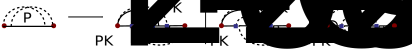
\includegraphics{KnottyPF/recursionP}
\end{equation}

where, generically, fragments $\PKnone^1\constr$ and $\PKnone^2\constr$ are decomposed into fragments $\PXnone$ and $\WPnone$ to account unambiguously for recursive substructure, such that we finally decompose $P$-fragments as follows:

\begin{equation}
\raisebox{36pt}{\text{$P$-structure}
=}
\begin{GRule}
\Pdecomposition{}
\end{GRule}
%\label{eq:pdecomposition}
\end{equation}

The rules for doing this efficiently are:

%\begin{equation}
%
\includegraphics{KnottyPF/recursionPK12}
%\end{equation}
\begin{GRule}
  \GRgapfragDeco{$\PKnone^1\constr$}{}{}
  \GRdecompTo
  \GRgapfragWDecompJ{$\PXnone$}{}{}{$\WPnone$}
\end{GRule}
\qquad
\begin{GRule}
  \GRgapfragDeco{$\PKnone^2\constr$}{}{}
  \GRdecompTo
  \GRgapfragWDecompK{$\PKnone^1\constr$}{}{}{$\WPnone$}
\end{GRule}

 

\begin{definition}
The structures represented by a $P_X$-rule over gapped region $[i..j]\cup [k..l]$ satisfy the following properties:
\begin{itemize}
\item all ends $i$, $j$, $k$, and $l$ are paired, but not necessarily to each other.
\item the closing bases at the ``$X$'' side of the gapped region form a base pair%``closed at $X$''
---there is a base pair at the position $X$ ($X\in\{L,R,M,O\}$).
\item there is a base pair that spans the gapped region $j+1..k-1$
\item unless $X=O$, the end bases cannot all be part of the same band (i.e. $i=j$ and $k=l$). (Note that we terminate with \Ob, unlike the original CCJ recursions, which terminate at \Mb.)
\end{itemize}
\end{definition}


%We obtain the following decompositions of $PK$-fragments\SW{which are now degenerated and should be short cut / removed} 
%%\begin{equation}
%%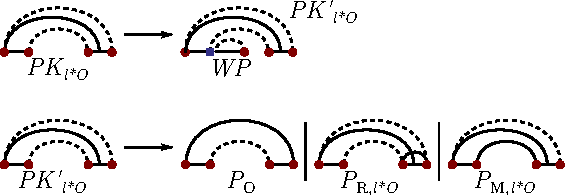
\includegraphics{KnottyPF/recursionPKlstarO}
%%\end{equation}
%
%\begin{equation}
%\begin{GRule}
%  \GRgapfragDeco{$\PKnone\constrIO$}{}{lO}
%  \GRdecompTo
%  \GRgapfragDeco{$\POnone$}{O}{}
%  %\GRor
%  %\GRgapfragDeco{$\PRnone\constrIO$}{R}{lO} 
%  %\GRor
%  %\GRgapfragDeco{$\PMnone\constrIO$}{M}{lO}
%
%  \GRnewrule
%
%  \GRgapfragDeco{$\PKnone\constrIL$}{}{oL}
%  \GRdecompTo
%  \GRgapfragDeco{$\PLnone$}{L}{}
%  %\GRor
%  %\GRgapfragDeco{$\PRnone\constrIL$}{R}{oL} 
%  %\GRor
%  %\GRgapfragDeco{$\PMnone\constrIL$}{M}{oL} 
%
%  \GRnewrule
%
%  \GRgapfragDeco{$\PKnone\constrIIO$}{}{rO}
%  \GRdecompTo
%  \GRgapfragDeco{$\POnone$}{O}{}
%  %\GRor
%  %\GRgapfragDeco{$\PLnone\constrIIO$}{L}{rO} 
%  %\GRor
%  %\GRgapfragDeco{$\PMnone\constrIIO$}{M}{rO} 
%
%  \GRnewrule
%
%  \GRgapfragDeco{$\PKnone\constrIIR$}{}{oR}
%  \GRdecompTo
%  \GRgapfragDeco{$\PRnone$}{R}{}
%  %\GRor
%  %\GRgapfragDeco{$\PLnone\constrIIR$}{L}{oR} 
%  %\GRor
%  %\GRgapfragDeco{$\PMnone\constrIIR$}{M}{oR} 
%\end{GRule}
%\end{equation}
%

We need to further decompose the $P_X$ fragments (which are optionally restricted by regular expressions). Generally, we distinguish three cases by the type of the closing base pair at position $X$. 1) it could close an interior loop in the same band, 2) a multi-loop in the same band (with costs for inner base pairs and unpaired based accounted in WB), or 3) it could `close' the band, i.e. it is the innermost base pair of its band for bands at L,R,O---outermost, in the case of M. Note that the decomposition is disjoint. In the
third case, one changes to decomposing some other band (or terminates the final O-band). Also, in the third case, we allow recursive substructure between bands (WP), which needs to be inserted unambiguously.

Let us first move the unambiguous decomposition of multi-loops within bands out of the way (where the recursions operate on gapped fragments). The recursions split of fragments $\WBnone$ and $\WBnone'$, which respecively describe general multi-loop fragments or such fragments with at least one base pair due to the following rules

\begin{equation}
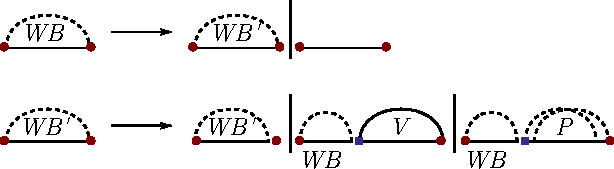
\includegraphics{KnottyPF/recursions-WB}
\end{equation}

Now, the complete rules for multi-loop decomposition within bands are:

\begin{align}
\begin{GRule}
  \GRgapfragDeco{$\PLnone{_\text{,mloop}}$}{L}{}
  \GRdecompTo
  \GRgapfragDeco[itype/.style={fix,shift={(-0.3,0)}},
                 jtype/.style={fix,shift={(+0.3,0)}}]
                {$\PLnone{_\text{,mloop00}}$}{fromL}{}
  % 
  \GRnewrule
  %
  \GRgapfragDeco{$\PLnone{_\text{,mloop10}}$}{L}{}
  \GRdecompTo
  \GRgapfragWDecompJ{$\PLnone$}{L}{}{$\WBnone$}
\end{GRule}\qquad
&
\begin{GRule}
  \GRgapfragDeco{$\PLnone{_\text{,mloop00}}$}{L}{}
  \GRdecompTo
  \GRgapfragWDecompI{$\PLnone{_\text{,mloop10}}$}{fromL}{}{$\WBnone'$}
  \GRor
  \GRgapfragWDecompJ{$\PLnone{_\text{,mloop01}}$}{fromL}{}{$\WBnone'$}
  %
  \GRnewrule
  %
  \GRgapfragDeco{$\PLnone{_\text{,mloop01}}$}{L}{}
  \GRdecompTo
  \GRgapfragWDecompI{$\PLnone$}{L}{}{$\WBnone$}
\end{GRule}
\\
\begin{GRule}
  \GRgapfragDeco{$\PMnone{_\text{,mloop}}$}{M}{}
  \GRdecompTo
  \GRgapfragDeco[ktype/.style={fix,shift={(-0.3,0)}},
                 jtype/.style={fix,shift={(+0.3,0)}}]
                {$\PMnone{_\text{,mloop00}}$}{fromM}{}
  % 
  \GRnewrule
  %
  \GRgapfragDeco{$\PMnone{_\text{,mloop10}}$}{M}{}
  \GRdecompTo
  \GRgapfragWDecompJ{$\PMnone$}{M}{}{$\WBnone$}
\end{GRule}\qquad
&
\begin{GRule}
  \GRgapfragDeco{$\PMnone{_\text{,mloop00}}$}{M}{}
  \GRdecompTo
  \GRgapfragWDecompI{$\PMnone{_\text{,mloop10}}$}{fromM}{}{$\WBnone'$}
  \GRor
  \GRgapfragWDecompJ{$\PMnone{_\text{,mloop01}}$}{fromM}{}{$\WBnone'$}
  %
  \GRnewrule
  %
  \GRgapfragDeco{$\PMnone{_\text{,mloop01}}$}{M}{}
  \GRdecompTo
  \GRgapfragWDecompK{$\PMnone$}{M}{}{$\WBnone$}
\end{GRule}
\end{align}

The corresponding rules with constraints look exactly like the unconstrained rules, but pass through the constraint.

It remains to ensure that the order in which bands are decomposed is never ambiguous. Note that in the handling of interior loops and multi-loops within a band, we can simply pass through any constraints on the order of band-decompositions.

\paragraph{Unambiguous decomposition order:}
The original CCJ algorithm already contains restrictions on the band-decomposition order, which are encoded in the rules for decomposition of $P\text{fromX}$-fragments ($X$ in $\{\text{L,R,M,O}\}$). These restrictions are
\begin{itemize}
\item (decomposition at) \Rb{} cannot be immediately followed by \Lb
\item \Mb{} cannot be immediately followed by \Ob{} 
\item \Ob{} cannot be immediately followed by \Mb
\end{itemize} 

The first restriction is indeed a disambiguation, since immediately successive decompositions at \Lb{} and \Rb{} could be exchanged, but it is again required to ensure that position changes introduce band changes, since going back and forth between \Lb{} and \Rb{} like $LRL$ would just extend the \Lb{} band. 


Here are the decomposition of $P_X$ without constraints.

Note that for resolving ambiguity, we introduce extra matrices $\POSnone$ and $\POnone$ where single O-band is respectively enforced or forbidden. This is later used to rule out transitions from \Mb{} to single \Ob-band, which would otherwise not result in a true change of bands and introduce ambiguity.

\begin{equation}
\begin{GRule}
  \GRgapfragDeco{$\PLnone$}{L}{}
  \GRdecompTo
  \GRgapfragDeco{$\PLnone{_{\text{,iloop}}}$}{L}{}
  \GRor
  \GRgapfragDeco{$\PLnone{_{\text{,mloop}}}$}{L}{}
  \GRor
  \GRgapfragDeco[itype/.style={fix,shift={(-0.3,0)}},
                 jtype/.style={fix,shift={(+0.3,0)}}]{$\PfromLnone$}{fromL}{}

  \GRnewrule

  \GRgapfragDeco{$\PMnone$}{M}{}
  \GRdecompTo
  \GRgapfragDeco{$\PMnone{_{\text{,iloop}}}$}{M}{}
  \GRor
  \GRgapfragDeco{$\PMnone{_{\text{,mloop}}}$}{M}{}
  \GRor
  \GRgapfragDeco[ktype/.style={fix,shift={(-0.3,0)}},
                 jtype/.style={fix,shift={(+0.3,0)}}]{$\PfromMnone$}{fromM}{}

  \GRnewrule

  \GRgapfragDeco{$\PRnone$}{R}{}
  \GRdecompTo
  \GRgapfragDeco{$\PRnone{_{\text{,iloop}}}$}{R}{}
  \GRor
  \GRgapfragDeco{$\PRnone{_{\text{,mloop}}}$}{R}{}
  \GRor
  \GRgapfragDeco[ktype/.style={fix,shift={(-0.3,0)}},
                 ltype/.style={fix,shift={(+0.3,0)}}]{$\PfromRnone$}{fromR}{}

  \GRnewrule

  \GRgapfragDeco{$\POSnone$}{O}{}
  \GRdecompTo
  \GRgapfragDeco{$\POSnone{_{\text{,iloop}}}$}{O}{}
  \GRor
  \GRgapfragDeco{$\POSnone{_{\text{,mloop}}}$}{O}{}
  \GRor
  \GRsingleOfrag
  
  \GRnewrule

  \GRgapfragDeco{$\POMnone$}{O}{}
  \GRdecompTo
  \GRgapfragDeco{$\POMnone{_{\text{,iloop}}}$}{O}{}
  \GRor
  \GRgapfragDeco{$\POMnone{_{\text{,mloop}}}$}{O}{}
  \GRor
  \GRgapfragDeco[itype/.style={fix,shift={(-0.3,0)}},
                 ltype/.style={fix,shift={(+0.3,0)}}]{$\PfromOnone$}{fromO}{}

  \GRnewrule
  \GRgapfragDeco{$\POnone$}{O}{}
  \GRdecompTo
  \GRgapfragDeco{$\POSnone$}{O}{}
  \GRor
  \GRgapfragDeco{$\POMnone$}{O}{}
\end{GRule}
\end{equation}

$P_{fromX}$-fragments are required to change the band; note that we need to decompise recursive substructure unambiguously \emph{and} allow unambiguous band change. 
Note that recursive substructure from different fromX-matrices cannot be decomposed in different ways.

The unambiguous splitting off of recursive substructure when changing between bands requires to split off the structure left and right of the source band in sequential order. To keep the complexity low, one would introduce an additional matrix in a DP; to indicate this, we use symbols $\PfromXnone'$ and $\PfromXnone''$ (the latter is not necessarily materialized as matrix by DP algorithms).

The fromX rules express the allowed transitions between band decompositions; currently, we list only the transitions for the 'standard' cases, i.e. without the additional constraints on band ordering as explained in the next section. Compare this to the transition diagram of Eq.~\ref{eq:transitions}.

\begin{equation}
\begin{GRule}
  % fromO
  \GRgapfragDeco{$\PfromOnone$}{fromO}{}
  \GRdecompTo
  \GRgapfragWDecompI{$\PfromOnone'$}{fromO}{}{$\WPnone$}

  \GRsetlast[1]{l}

  \GRgapfragDeco{$\PfromOnone'$}{fromO}{}
  \GRdecompTo
  \GRgapfragWDecompL{$\PfromOnone''$}{fromO}{}{$\WPnone$}

  \GRnewrule

  \GRgapfragDeco{$\PfromOnone''$}{fromO}{}
  \GRdecompTo
  \GRgapfragDeco{$\PLnone$}{L}{}
  \GRor
  \GRgapfragDeco{$\PRnone$}{R}{}

  \GRnewrule

  % fromL
  \GRgapfragDeco{$\PfromLnone$}{fromL}{}
  \GRdecompTo
  \GRgapfragWDecompI{$\PfromLnone'$}{fromL}{}{$\WPnone$}
  %
  \GRsetlast[1]{l}
  \GRgapfragDeco{$\PfromLnone'$}{fromL}{}
  \GRdecompTo
  \GRgapfragWDecompJ{$\PfromLnone''$}{fromL}{}{$\WPnone$}
  %
  \GRnewrule
  \GRgapfragDeco{$\PfromLnone''$}{fromL}{}
  \GRdecompTo
  \GRgapfragDeco{$\PMnone$}{M}{}
  \GRor        
  \GRgapfragDeco{$\POnone$}{O}{}
  \GRor
  \GRgapfragDeco{$\PRnone$}{R}{}
  
  \GRnewrule

  % fromR
  \GRgapfragDeco{$\PfromRnone$}{fromR}{}
  \GRdecompTo
  \GRgapfragWDecompK{$\PfromRnone'$}{fromR}{}{$\WPnone$}
  \GRsetlast[1]{last}
  \GRgapfragDeco{$\PfromRnone'$}{fromR}{}
  \GRdecompTo
  \GRgapfragWDecompL{$\PfromRnone''$}{fromR}{}{$\WPnone$}

  \GRnewrule
  \GRgapfragDeco{$\PfromRnone''$}{fromR}{}
  \GRdecompTo
  \GRgapfragDeco{$\PMnone$}{M}{}
  \GRor        
  \GRgapfragDeco{$\POnone$}{O}{}
  %
  \GRnewrule
  \GRgapfragDeco{$\PfromMnone$}{fromM}{}     
  \GRdecompTo
  \GRgapfragWDecompJ{$\PfromMnone'$}{fromM}{}{$\WPnone$}
  \GRsetlast[1]{last}
  \GRgapfragDeco{$\PfromMnone'$}{fromM}{}     
  \GRdecompTo
  \GRgapfragWDecompK{$\PfromMnone''$}{fromM}{}{$\WPnone$}

  \GRnewrule
  \GRgapfragDeco{$\PfromMnone'$}{fromM}{}     
  \GRdecompTo
  \GRgapfragDeco{$\PLnone$}{L}{}
  \GRor
  \GRgapfragDeco{$\PRnone$}{R}{}
  \GRor
  \GRgapfragDeco{$\POMnone$}{O}{}
\end{GRule}
\end{equation}

%\begin{center}
%\begin{tikzpicture}[thick]
%\newcommand{\pkpre}{2}
%\newcommand{\classdist}{3.5}
%
%%mark O as terminal state
%\node (O) at (0,0) [circle,draw] {O};
%\draw (O) circle [thick,radius=0.28];
%
%\path (O)
%      +  (0,-1) node (Om) {Om}
%      ++ (\classdist,0) node (M) {M}
%      ++ (\classdist,0) node (L) {L}
%      ++ (\classdist,0) node (R) {R};
%
%
%\path (O) ++ (0,1) node (RlO) {R\constrIO}
%      ++(0,1) node (MlO) {M\constrIO};
%
%\path (M) ++ (0,1) node (LrO) {L\constrIIO}
%      ++ (0,1) node (MrO) {M\constrIIO};
%
%\path (L) ++ (0,1) node (MoL) {M\constrIL}
%      ++ (0,1) node (RoL) {R\constrIL};
%
%\path (R) ++ (0,1) node (MoR) {M\constrIIR}
%          ++ (0,1) node (LoR) {L\constrIIR};
%\draw
%  (MlO) edge [<->] (RlO)
%  (RlO) edge [->] (O)
%  (RoL) edge [<->] (MoL)
%  (MoL) edge [->] (L)
%%
%  (MrO) edge [<->] (LrO)
%  (LrO) edge [->] (O)
%  (LoR) edge [<->] (MoR)
%  (LoR) edge [->,out=330,in=40] (R)
%  (MoR) edge [->] (R)
%%
%  (R) edge [<->,out=210,in=330] (O)
%  (R) edge [<->,out=200,in=340] (M)
%  (L) edge [->] (R)
%  (L) edge [<->] (M)
%  (L) edge [<->,out=200,in=340] (O)
%  (O) edge [->] (M)
%  (Om) edge [->] (M) edge [->] (R) edge [->] (L);
%
%%PK init states
%\path[red] (O) ++(-\pkpre,1) node (PKlO) {\PKnone\constrIO}
%          ++(-0.3,1) node (start) {} 
%      (start) edge [->] (PKlO) 
%      (PKlO) edge [->] (Om)
%             edge [->] (RlO)
%             edge [->] (MlO);
%
%\path[red] (L) ++(-\pkpre,1) node (PKoL) {\PKnone\constrIL}
%          ++(-0.3,1) node (start) {} 
%      (start) edge [->] (PKoL) 
%      (PKoL) edge [->] (L)
%             edge [->] (RoL)
%             edge [->] (MoL);
%
%\path[red] (M) ++(-\pkpre,1) node (PKrO) {\PKnone\constrIIO}
%          ++(-0.3,1) node (start) {} 
%      (start) edge [->] (PKrO) 
%      (PKrO) edge [->] (Om)
%             edge [->] (LrO)
%             edge [->] (MrO);
%
%\path[red] (R) ++(-\pkpre,1) node (PKoR) {\PKnone\constrIIR}
%          ++(-0.3,1) node (start) {} 
%      (start) edge [->] (PKoR) 
%      (PKoR) edge [->] (R)
%             edge [->] (LoR)
%             edge [->] (MoR);
%\end{tikzpicture}
%\end{center}

Note that there is no transition from \Mb{} to the terminal state $Os$, which represents the decomposition of the singleton \Ob-band. Such a transition would lead to wrong scoring and ambiguity. Otherwise, transition from \Mb{} to the singleton \Ob-band is the only forbidden transition from \Mb{} to \Ob-band! This is the reason for introducing the $Os$-states in the first place.  

%Probably not necessary anymore:
%\SW{Idea: We should formally define \emph{band decomposition order (BDO)} (as a word over $\{L,R,M,O\}$ for decompositions of a structure
%represented by $P$. Proving the uniqueness of BDO (given our restrictions) would be an essential step to showing the uniqueness of the recursions. For showing completeness, it is important to precisely define all the fragments (in terms of the represented structures).}

\newpage
\section{Systematic restart}
\label{sec:pdecomposition}

\newcommand{\CGR}{CGR} %% closed gapped structures
\newcommand{\CR}{CR}   %% closed (ungapped) structures
    

An RNA sequence is a word over $\{A,C,G,U\}.$
\textbf{HJ-} Each character is defined as a base and is referred to by its index. Index starts from 0?
The pairs of bases (A,U), (C,G), (G,C), (G,U), (U,A), and (U,G) are said to be complementary base pairs.
A base pair for an RNA sequence $S$ with length $n$ is an ordered pair $i.l$ with $1 \leq i <l \leq n$, such that $i$th and $l$th bases of $S$ are complementary. $i$ and $l$ are called the endpoints of the base pair. 

A \emph{region} is a set of positive integers, the positions of the region \SW{define and distinguish gapped and ungapped regions}. \textbf{HJ-} here we can just place the definitions of region and gapped region as in section 1.1.

An \emph{RNA secondary structure over the region $r$} is a set of base pairs $i.j$ of positions of $r$, such that for all base pairs $i.j$, $i'.j'$ of the structure,
$|\{i,j\}\cap\{i',j'\}|\neq 1.$


In the following, we define bands and band decomposition orders of closed structures over gapped regions (\CGR-structures). This leads to defining decomposition orders, which characterize subsets of those structures.

The \emph{maximal bands} of an RNA structure over a region are the regions that are closed by the base pairs at the ends of a maximal chain of immediately nested base pairs that all have the same crossing pattern to the base pairs in the structure. Here two base pairs in a structure are \emph{immediately nested}, iff they are nested and their is no other base pair that is nested in the outer base pair and enclosing the inner base pair. \SW{This description of bands is probably too informal!}

\emph{Recursive substructure} of a structure over a region is a structure over a connected subregion in the region, where no base pair of the structure has one end in the subregion and one base pair outside of the subregion.

A \emph{\CGR-structure} over the gapped region $[i,j]\cup[k,l]$ is a structure $R$ over this region iff
\begin{itemize}
  \item $R$ contains a base pair that spans the region, i.e. there is a base pair $x.y\in R$, where $x\in[i,j]$ and $y\in[k,l]$;
  \item At least two of the positions $i,j,k,$ and $l$ are paired to each other by $R$ and
    none of these positions is part of recursive substructure of $R$.
  \item Unless the region is a single band of the structure $R$, the structure 
    can be decomposed into the maximal band containing this base pair;
    potential recursive substructure involving either index $i,j,k,l$; 
    and a CGR structure.
\end{itemize}
For a \CGR-structure $R$, we call a band of $R$ an \Ob-band, if it contains $i.l$; \Lb-band, $i.j$; \Rb-band, if $k.l$; and otherwise \Mb-band, if it contains $j.k$ and is not an \Ob-band.

A band decomposition order (BDO) of a \CGR-structure is a sequence over $\{O,L,R,M\}$, such that the structure can be decomposed by iterative decomposition into $X$-bands $X \in \{O,L,R,M\}$, (and remaining structure) in the order of the BDO.
To avoid obvious ambiguity in BDOs, we restrict BDOs additionally by forbidding the subwords RL and OM. Note that BDOs of structures, do not contain homo-$q$-mers, $q\geq 2$ and cannot end in $MO$, due to maximality of the split-off bands. BDOs must end in \Ob{}.

Claim: There is a single, uniquely determined  BDO for each \CGR-structures.

Proofsketch: Each \CGR-structure either corresponds to a single (O-)band, or can be decomposed into at least one X-band, potentially recursive substructure and a remaining \CGR-structure. If a decomposition is as well possible for a $Y$-band, $X\neq Y$, then either $X,Y\in\{L,R\}$ or $X,Y\in\{M,O\}$. In these cases, the ambiguity is broken by forbidding subwords RL and OM. Since this enforces to start the decomposition with respectively LR or MO, this breaks all remaining ambiguity. More elaborately, this could be shown by induction over the length of the BDO.\\
\textbf{HJ-} Should we say at all that the decomposition has an order, say from left to right of the RNA structure over the region?

For a regular expression $x$ over alphabet $\{O,L,M,R\}$, we define \emph{$CGR_x$-fragments over the region $[i,j]\cup[k,l]$}, whose structures are exactly the \CGR-structures with BDOs that start with the decomposition described by $x$.

We consider closed structures over regions $[i,l]$ (\CR) as structures that are decomposable into two \CGR-structures and recursive substructures due to
$$
\begin{GRule}
\Pdecomposition{}
\end{GRule}
$$
and where all occurring recursive substructure are \CR-structures; idea: CCJ-structures are the structures that (unless they are non-crossing) can be decomposed into a sequence of \CR-structures and recursive substructures, which are CCJ-structures (compare $W$-rule, Eq.~\ref{eq:wrule})

We define the set of closed structures $\CR_{x/y}$ that are decomposable into 
a $\CGR_x$-structure over $[i_1,j_1]\cup[k_1,l_1]$ and
a $\CGR_y$-structure over $[i_2,j_2]\cup[k_2,l_2]$.
%
We observe the following equivalences (due to flipping bands from the first gapped fragment to the second one):
\begin{itemize}
  \item $\CR_{Mx/y}=\CR_{x/Ly}$
  \item $\CR_{Rx/y}=\CR_{x/My}$
\end{itemize}
We can thus shift all middle and right bands from the first to the second gapped fragment, maintaining equivalence and avoiding ambiguity; in graphical notation:%
\begin{equation}
% M -> L
\begin{GRule}
  \GRgapfragCoordinates{0.6}{0.6}
  \GRgapfragEatBandM[red,very thick]{}
  \GRgapfragArcs[thin]{}
  \draw[solid,thick] (i) -- (j) (k) -- (l);

  \GRsetlast[0.1]{j}
  \begin{scope}[yscale=-1]
    \GRgapfragCoordinates{0.6}{0.7}
    \GRgapfragEatBandL[draw=none]{}
    \GRgapfragArcs[thin]{}
    \draw[solid,thick] (i) -- (j) (k) -- (l);
    \GRsetlast{l}
  \end{scope}

  \GRdecompTo

  \GRgapfragCoordinates{0.6}{0.6}
  \GRgapfragEatBandM[draw=none]{}
  \GRgapfragArcs[thin]{}
  \draw[solid,thick] (i) -- (j) (k) -- (l);
  \GRsetlast[0.1]{j}
  \begin{scope}[yscale=-1]
    \GRgapfragCoordinates{0.6}{0.7}
    \GRgapfragEatBandL[red,very thick]{}
    \GRgapfragArcs[thin]{}
    \draw[solid,thick] (i) -- (j) (k) -- (l);
  \end{scope}
\end{GRule}
\qquad
% R -> M
\begin{GRule}
  \GRgapfragCoordinates{0.6}{0.7}
  \GRgapfragEatBandR[red,very thick]{}
  \GRgapfragArcs[thin]{}
  \draw[solid,thick] (i) -- (j) (k) -- (l);

  \GRsetlast[0.1]{j}
  \begin{scope}[yscale=-1]
    \GRgapfragCoordinates{0.6}{0.6}
    \GRgapfragEatBandM[draw=none]{}
    \GRgapfragArcs[thin]{}
    \draw[solid,thick] (i) -- (j) (k) -- (l);
    \GRsetlast{l}
  \end{scope}

  \GRdecompTo

  \GRgapfragCoordinates{0.6}{0.7}
  \GRgapfragEatBandR[draw=none]{}
  \GRgapfragArcs[thin]{}
  \draw[solid,thick] (i) -- (j) (k) -- (l);
  \GRsetlast[0.1]{j}
  \begin{scope}[yscale=-1]
    \GRgapfragCoordinates{0.6}{0.6}
    \GRgapfragEatBandM[red,very thick]{}
    \GRgapfragArcs[thin]{}
    \draw[solid,thick] (i) -- (j) (k) -- (l);
  \end{scope}
\end{GRule}
  \label{eq:band-shift}
\end{equation}
%
Consequently, in the decomposition of CR-structures, we consider only those first gapped fragments that start with \Ob{} or \Lb. For completeness, we do not restrict the second fragment in this way.

    TODO: define \emph{exposed} L,R,M,O band


In the decomposition of closed ungapped fragments, we need to rule out all cases,
where the first fragment has an exposed \Mb-band and the second has exposed \Lb-band,
since they would split a band of the joint structure (which would cause ambiguity and lead to miscounting the number of band and band changes).
Analogously, this happens for exposed \Rb-band in fragment one and \Mb-band in fragment two.

Note we limit the band decomposition order, such that start in \Ob{} rules out exposed \Mb-band; as well, start in \Rb{} rules out exposed \Lb{}.   
Thus, the only remaining band splitting case is 
$$\CR_{\Lb\Rb{}x/\Mb{}y} =
\begin{GRule}
  \GRgapfragCoordinates{0.6}{0.7}
  \GRgapfragEatBandL[red,very thick]{}
  \GRgapfragEatBandR[red,very thick]{}
  \GRgapfragArcs[thin]{}
  \draw[solid,thick] (i) -- (j) (k) -- (l);

  \GRsetlast[0.2]{j}
  \begin{scope}[yscale=-1]
    \GRgapfragCoordinates{0.6}{0.6}
    \GRgapfragEatBandM[draw=none]{}
    \GRgapfragEatBandM[red,very thick]{}
    \GRgapfragArcs[thin]{}
    \draw[solid,thick] (i) -- (j) (k) -- (l);
    \GRsetlast{l}
  \end{scope}
\end{GRule}
$$
This can be fixed by forbidding exposed middle band (corresponding to start in $\Mb$) for the second fragment, if the first fragment starts with $\Lb$.

Furthermore, there is ambiguity in how the chains of crossing base pairs that transitively connect the left end to the right end of a $\CR$-structure can be distributed over the first and second gapped fragment.
In the case of three-chains, there is ambiguity due to:

\begin{equation}
\begin{GRule}
  \GRgapfragCoordinates{0.6}{0.8}
  \GRgapfragEatBandO[red,very thick]{}
  \GRgapfragArcs[thin]{}
  \draw[solid,thick] (i) -- (j) (k) -- (l);

  \GRsetlast[0.1]{j}
  \begin{scope}[yscale=-1]
    \GRgapfragCoordinates{0.6}{0.8}
    \GRgapfragEatBandR[red,very thick]{}
    \GRgapfragEatBandO[red,very thick]{}
    \GRgapfragArcs[thin]{}
    \draw[solid,thick] (i) -- (j) (k) -- (l);
    \GRsetlast{l}
  \end{scope}
\end{GRule}
\qquad
\begin{GRule}
  \GRgapfragCoordinates{0.6}{0.8}
  \GRgapfragEatBandL[red,very thick]{}
  \GRgapfragEatBandO[red,very thick]{}
  \GRgapfragArcs[thin]{}
  \draw[solid,thick] (i) -- (j) (k) -- (l);

  \GRsetlast[0.2]{j}
  \begin{scope}[yscale=-1]
    \GRgapfragCoordinates{0.6}{0.8}
    \GRgapfragEatBandO[red,very thick]{}
    \GRgapfragArcs[thin]{}
    \draw[solid,thick] (i) -- (j) (k) -- (l);
    \GRsetlast{l}
  \end{scope}
\end{GRule}
\end{equation}

However, as Yann pointed out, these decompositions are not obviously equivalent! \SW{We have a problem here! Could this be fixed by decomposing 3-chains into one gapped fragment + recursive substructure? Problem there: 3-chain structures from two gapped structure can contain more than three groups of bands! Also: not all such structures are original CCJ-structures, since they are too interlocked to be split into two structures over gapped fragments! Is there an unwanted subtlety in the CCJ-recursions?}

Due to the above considerations, we handle the disjoint cases of two-chains, three-chains and four-chains separately:

\newcommand{\GRfragLabel}[2][]{%
  \path (i) -- node [below,#1] {#2} (l);
}

\def\tokenize#1{\ifx#1\tokenize\else#1{, }\expandafter\tokenize\fi}

\newcommand{\GRgapfragBandEater}[1]{%
  \GRgapfragCoordinates{0.8}{0.7}
  \foreach \x in {#1}{%
    \csname GRgapfragEatBand\x \endcsname[red,very thick]{}%
  }
  \GRgapfragArcs[thin]{}
  \draw[solid,thick] (i) -- (j) (k) -- (l);
  \GRfragLabel{#1}
}
  
\begin{itemize}
  \item 
    In the case of two-chains, the (BDO of the) first fragment needs to start with \Ob-band, such that the base pair from the left most index of the structure spans the region. Moreover, the base pair from the right most index in the second gapped fragment has to span the region. We guarantee this, by limiting the BDO-prefix of the second fragment by the regular expression $[L,M]^*\Ob$. Here are examples of allowed second fragment prefix decomposition:
   \begin{equation}
\begin{GRule}
  \GRgapfragCoordinates{0.8}{0.7}
  \GRgapfragEatBandO[red,very thick]{}
  \GRgapfragArcs[thin]{}
  \draw[solid,thick] (i) -- (j) (k) -- (l);
  \GRfragLabel{O}

  \GRsetlast[1]{l}
  \GRgapfragBandEater{M, L, O}
%  \GRgapfragEatBandM[red,very thick]{}
%  \GRgapfragEatBandL[red,very thick]{}
%  \GRgapfragEatBandO[red,very thick]{}

  \GRsetlast[1]{l}

  \GRgapfragCoordinates{0.8}{0.7}
  \GRgapfragEatBandL[red,very thick]{}
  \GRgapfragEatBandM[red,very thick]{}
  \GRgapfragEatBandO[red,very thick]{}
  \GRgapfragArcs[thin]{}
  \draw[solid,thick] (i) -- (j) (k) -- (l);
  \GRfragLabel{LMO}

  \GRsetlast[1]{l}

  \GRgapfragCoordinates{0.8}{0.7}
  \GRgapfragEatBandL[red,very thick]{}
  \GRgapfragEatBandM[red,very thick]{}
  \GRgapfragEatBandL[red,very thick]{}
  \GRgapfragEatBandM[red,very thick]{}
  \GRgapfragEatBandO[red,very thick]{}
  \GRgapfragArcs[thin]{}
  \draw[solid,thick] (i) -- (j) (k) -- (l);
  \GRfragLabel{LMLMO}
\end{GRule}
    \end{equation}
  \item
    In the case of three-chains, we limit the BDO of the first gapped fragment to prefix \Ob{} and the second gapped fragment to $[L,M]^*\Rb$.
Examples:
   \begin{equation}
\begin{GRule}
  \GRgapfragCoordinates{0.8}{0.7}
  \GRgapfragEatBandR[red,very thick]{}
  \GRgapfragArcs[thin]{}
  \draw[solid,thick] (i) -- (j) (k) -- (l);
  \GRfragLabel{R}

  \GRsetlast[1]{l}

  \GRgapfragCoordinates{0.8}{0.7}
  \GRgapfragEatBandM[red,very thick]{}
  \GRgapfragEatBandL[red,very thick]{}
  \GRgapfragEatBandR[red,very thick]{}
  \GRgapfragArcs[thin]{}
  \draw[solid,thick] (i) -- (j) (k) -- (l);
  \GRfragLabel{MLR}

  \GRsetlast[1]{l}
  \GRgapfragCoordinates{0.8}{0.7}
  \GRgapfragEatBandL[red,very thick]{}
  \GRgapfragEatBandM[red,very thick]{}
  \GRgapfragEatBandR[red,very thick]{}
  \GRgapfragArcs[thin]{}
  \draw[solid,thick] (i) -- (j) (k) -- (l);
  \GRfragLabel{LMR}

  \GRsetlast[1]{l}

  \GRgapfragCoordinates{0.8}{0.7}
  \GRgapfragEatBandL[red,very thick]{}
  \GRgapfragEatBandM[red,very thick]{}
  \GRgapfragEatBandL[red,very thick]{}
  \GRgapfragEatBandM[red,very thick]{}
  \GRgapfragEatBandR[red,very thick]{}
  \GRgapfragArcs[thin]{}
  \draw[solid,thick] (i) -- (j) (k) -- (l);
  \GRfragLabel{LMLMR}
\end{GRule}
    \end{equation}

  \item Only in the case of four-chains we use $\CGR_\Lb$ for the first fragment. The second fragment is constrained like in the case of three chains, where we additionally need to avoid exposing the \Mb-band. Thus, we restrict it by $\Lb[\Lb,\Mb]^*\Rb | \Rb$.
Examples:
   \begin{equation}
\begin{GRule}
  \GRgapfragCoordinates{0.8}{0.7}
  \GRgapfragEatBandR[red,very thick]{}
  \GRgapfragArcs[thin]{}
  \draw[solid,thick] (i) -- (j) (k) -- (l);
  \GRfragLabel{R}

  \GRsetlast[1]{l}

  \GRgapfragCoordinates{0.8}{0.7}
  \GRgapfragEatBandL[red,very thick]{}
  \GRgapfragEatBandR[red,very thick]{}
  \GRgapfragArcs[thin]{}
  \draw[solid,thick] (i) -- (j) (k) -- (l);
  \GRfragLabel{LR}

  \GRsetlast[1]{l}

  \GRgapfragCoordinates{0.8}{0.7}
  \GRgapfragEatBandL[red,very thick]{}
  \GRgapfragEatBandM[red,very thick]{}
  \GRgapfragEatBandR[red,very thick]{}
  \GRgapfragArcs[thin]{}
  \draw[solid,thick] (i) -- (j) (k) -- (l);
  \GRfragLabel{LMR}

  \GRsetlast[1]{l}

  \GRgapfragCoordinates{0.8}{0.7}
  \GRgapfragEatBandL[red,very thick]{}
  \GRgapfragEatBandM[red,very thick]{}
  \GRgapfragEatBandL[red,very thick]{}
  \GRgapfragEatBandR[red,very thick]{}
  \GRgapfragArcs[thin]{}
  \draw[solid,thick] (i) -- (j) (k) -- (l);
  \GRfragLabel{LMLR}
\end{GRule}
    \end{equation}
\end{itemize}

Here is the fragment decomposition transition diagram coming out of the above considerations:
%
\begin{equation}
\label{eq:transitions}
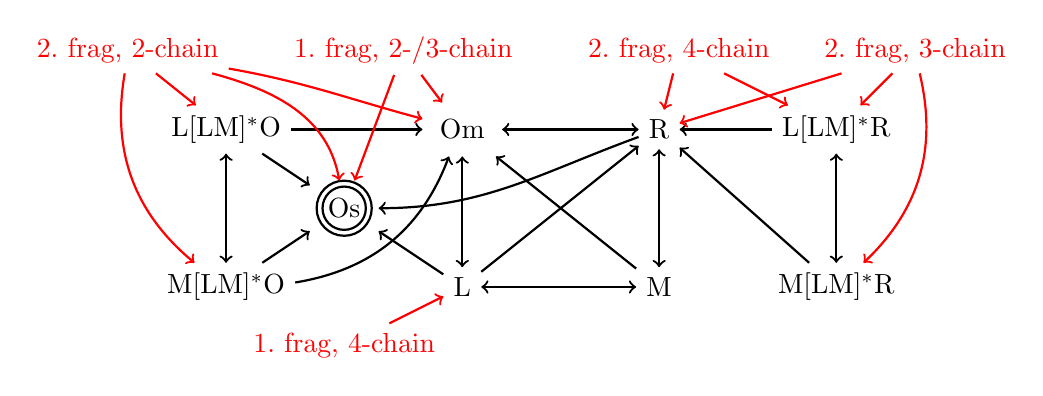
\begin{tikzpicture}[thick]
\newcommand{\pkpre}{2}
\newcommand{\classdist}{2.5}

%mark O as terminal state
\path (0,0) node (Om) [outer sep=3] {Om}
      +  (-1.5,-1) node (Os) [outer sep=3.25] {Os}
      + (\classdist,0) node (R) {R}
      + (0,-2) node (L) {L}
      + (\classdist,-2) node (M) {M};

\draw (Os) circle [thick,radius=0.275];
\draw (Os) circle [thick,radius=0.35];

\draw
  (R) edge [<->] (Om)
  edge [->,in=0,out=200] (Os)
  (R) edge [<->] (M)
  (L) edge [->] (R)
      edge [->] (Os)
  (L) edge [<->] (M)
  (L) edge [<->] (Om)
  (M) edge [->] (Om);


\path (-3,0) node (LLMsO) {$\Lb[\Lb\Mb]^*\Ob$}
      +(0,-2) node (MLMsO) {$\Mb[\Lb\Mb]^*\Ob$}
      (4.75,0) node (LLMsR) {$\Lb[\Lb\Mb]^*\Rb$}
      +(0,-2) node (MLMsR) {$\Mb[\Lb\Mb]^*\Rb$};

\draw (LLMsO) edge [<->] (MLMsO)
      (LLMsR) edge [<->] (MLMsR)
      (LLMsO) edge [->] (Os) edge [->] (Om)
      (MLMsO) edge [->] (Os) edge [->,bend right] (Om)
      (LLMsR) edge [->] (R)
      (MLMsR) edge [->] (R);

% draw start arrows
\draw[red]
  (Os) ++ (0.75,2) node {1.~frag, 2-/3-chain} edge [->] (Om)
  edge [->] (Os)
  (L) ++ (-1.5,-0.75) node {1.~frag, 4-chain} edge [->] (L)
  (R) ++ (0.25,1) node {2.~frag, 4-chain} edge [->] (LLMsR) edge [->] (R)
  (LLMsO) ++ (-1.25,1) node {2.~frag, 2-chain} 
  edge [->] (LLMsO) edge [->,bend right] (MLMsO) edge [->,out=345,in=100] (Os) edge [->,out=350,in=165] (Om)
  (LLMsR) ++ (1,1) node {2.~frag, 3-chain} 
  edge [->] (LLMsR) edge [->,bend left] (MLMsR) edge [->] (R);

\end{tikzpicture}
\end{equation}


\textbf{HJ-} In CCJ we start decomposition from left to right with a predefined BDO. I am wondering if that could have been used here. \SW{I need some more explanations:). I think we already use left to right decomposition, don't we?}

---------------------------

%\renewcommand{\P}{{\cal P}}

%Let $\P$ be the set of $P$-structures over $[i,l]$.

%Recall: These $P$-structures are the structures of a $P$-fragment (over region $[i,l]$), i.e. the structures that can be decomposed by the $P$-rule.

%\paragraph{Some simple truths:}
%\begin{enumerate}
%\item the ends in $P$-structures are paired; there are base pairs (i,i') and (l',l) in each $R\in \P$.
%\item the ends are not part of recursive substructure, i.e.\ there is a chain of crossing base pairs connecting the two ends.
%\item the chain has either length 2, 3, or 4; this leads to the disjoint decomposition
%$$\P = \P_2 \uplus \P_3 \uplus \P_4,$$
%where the $\P_i$ (i=2,3,4) are pairwise disjoint, and 
%\begin{enumerate}
%\item $\P_2 = \{R\in \P \mid \exists i',l': (i,i')\in R, (l',l)\in R, l'<i'\}$
%\item $\P_3 = \{R\in \P \mid \exists i',l',p,p': (i,i')\in R, (p,p')\in R, (l',l)\in R, p<i'<l'<p'\}$ 
%\item $\P_4 = \{R\in \P \mid \exists i',l',p,p',: (i,i')\in R, (p,p')\in R, (q,q')\in R, (l',l)\in R, p<i'<q<p'<l'<q'\}$.
%\end{enumerate}
%\item all $P$-structures can be decomposed into two $PK$-fragments (eventually, recursive substructure and two $\PXnone$-fragments)
%\item each structure of a $PK$-fragment contains one base pair that spans the region; there cannot be two such base pairs that cross each other
%\item each structure of a $PK$-fragment can be decomposed by a series of decompositions of bands at positions \Lb,\Mb,\Rb{},\Ob; in a non-ambiguous set of decomposition rules, there is exactly one order of decompositions for each structure.
%\item We can specify rules to decompose only structures from each of the single subclasses from specialized $PK$-fragments.
%\begin{enumerate}
%\item $\P_2$ is generated by requiring that in (all structures of) the first $PK$-fragment $(i,i')$ spans the gapped region; and in the second, (l',l) spans the gapped region.
%\item $\P_3$ is generated by requiring that in the first fragment $(i,i')$ spans the gapped region; and in the second, (l',l) does not span the gapped region.
%\item $\P_4$ is generated by requiring that in the first fragment $(i,i')$ does not span the gapped region; and in the second, (l',l) does not span the gapped region.
%\end{enumerate}
%\end{enumerate}

%\paragraph{Characterization of a $\PXnone$-fragment}
%While $PK$-fragments are used in the decomposition of $P$-fragments, there only purpose is to decompose $P$-fragments into a $P_X$ and a $P_Y$-fragment ($X,Y\in\{\Lb,\Rb,\Mb,\Ob\}$), while unambigously allowing recursive substructure.
%Thus, we should first of all characterize $P_X$ fragments in order to understand the $P$-decomposition.
%\begin{equation}
%\raisebox{36pt}{\text{$P$-structure}
%=}
%\begin{GRule}
%\Pdecomposition{}
%\end{GRule}
%\label{eq:pdecomposition}
%\end{equation}
%
%
%\begin{definition}[$\POnone$-structures]
%The structures of a $\POnone$-fragment, i.e. the $P_X$-structures, are the $PK$-structures $R$ over the fragment's region $[i,j]\cup[k,l]$, where
%\begin{itemize}
%\item $(i,l) \in R$
%\item $\exists j.j'\in R, k.k'\in R$ 
%\item if $(j,k)\in R$, then $R$ consists of a single band
%\item otherwise, $j.j'$ and $k.k'$ belong to different bands; one of them could be an \Ob-band. In this case, this must be the band of $(i,l)$.
%\end{itemize}
%\end{definition}
%
%\SW{define $\PLnone$, $\PRnone$, $\PMnone$-structures}
%\SW{define base pair at the X-position for a gapped region}
%
%\begin{proposition}
%The $\POnone$, $\PLnone$, $\PRnone$, $\PMnone$-structures over a region $[i,j]\cup[k,l]$ are disjoint.
%\end{proposition}
%\begin{proofsketch}
%  Each $\PXnone$-structure contains a (band closing) base pair at the $X$ position. Two base pairs in 
%  resptivee positions L or R and O or M are mutually exlcusive.
%  Moreover, we explicitely guarantee (in the recursions enforced by the possible band decomposition orders), 
%  that $\PLnone$-structures cannot have a base pair in position \Rb{}, 
%  and $\POnone$-structures cannot have a base pair in position \Mb. 
%\end{proofsketch}
%
%\begin{proposition}
%Each structure $R$ of $\P_2$ over region $[i,l]$ can be decomposed into recursive substructure and two $\POnone$-fragments over respective regions $[i_1,j_1]\cup[k_1,l_1]$ and $[i_2,j_2]\cup[k_2,l_2]$ such that $i=i_1$, $l=l_2$, $(i,l_1)\in R$, and $(i_2,l)\in R$.
%Furthermore, this decomposition is unambiguous.
%\end{proposition}
%
%\begin{proofsketch}
%Let $R$ be an arbitrary structure of region in $\P_2$ over $(i,l)$. Since $R$ is a $P$-structure there must be some decomposition into a $P_X$ structure, a $P_Y$ structure, and recursive substructure as in Eq.~$(\ref{eq:pdecomposition})$. 
%Since $R$ is a two-chain $P$-structure,
%there must exist uniquely determined $i'$ and $l'$ s.t. $(i,i')$ and $(l',l)$ are base pairs of $R$ and cross each other. (Moreover there are no other base pairs that cross both of such base pairs in $R$.)
%
%If we set $l_1=i'$ and $i_2=l'$ (which corresponds to decomposition into two $\PO$-structures), $R$ can be decomposed, i.e.~there exist 
%$j_1$,$k_1$,$j_2$,$k_2$, .... (To be shown; idea: similar to argument for non-crossing, only that here we allow at most one crossing!).
%
%Take any base pair of $R$. It can be either crossing $(i_1,l_1)$ or $(i_2,l_2$) or none of them.
%
%Set $j_1$ to the right-most end of any connected base pair left of $i_2$.\dots
%
%-----------------------
%
%In other words, all base pairs that cross $(i_2,l)$ must be in the region $[i,l_1]$; moreover, they cannot cross each other. The symmetric statement holds for base pair $(i,l_1)$ and region $[i_2,l]$.
%
%All base pairs that cross $(i,l_1)$ can be represented in the first $\POnone$-fragment; the same holds symmetrically for $(i_2,l)$.
%
% All base pair that cross neither of these two base pairs, must be part of either the first or the second region (i.e. $[i_1,j_1]\cup[k_1,l_1]$ or $[i_2,j_2]\cup[k_2,l_2]$).
%
%
%\end{proofsketch}
%
%\begin{proposition}
%Each structure $R$ of $\P_3$ over region $[i,l]$ can be decomposed into recursive substructure, a $\POnone$-fragment and a $\PLnone$-fragment over respective regions $[i_1,j_1]\cup[k_1,l_1]$ and $[i_2,j_2]\cup[k_2,l_2]$ such that $i=i_1$, $l=l_2$, $(i,l_1)\in R$, and $(i_2,l)\not\in R$. 
%\end{proposition}
%%\begin{proofsketch}
%%\end{proofsketch}
%%
%
%\begin{proposition}
%Each structure $R$ of $\P_4$ over region $[i,l]$ can be decomposed into recursive substructure, a $\POnone$-fragment and a $\PLnone$-fragment over respective regions $[i_1,j_1]\cup[k_1,l_1]$ and $[i_2,j_2]\cup[k_2,l_2]$ such that $i=i_1$, $l=l_2$, $(i,l_1)\not\in R$, and $(i_2,l)\not\in R$. 
%\end{proposition}
%
%\begin{proofsketch}
%\end{proofsketch}
%%%

\end{document}
